\documentclass{beamer}
\usepackage[utf8]{inputenc}
\usepackage[ngerman]{babel}
\usepackage{amssymb,amstext}
\usepackage{amsmath}
\usepackage{amsfonts}
\usepackage{graphicx}
\usepackage{pdfpages} 
\usepackage{subfigure} 
\usepackage{tcolorbox}
\usepackage{cases}
\usepackage{listings}
\usepackage[export]{adjustbox}
\title[Hubbard triangle]{Hubbard triangle}
\subtitle{Computational Material Science}
\author[A. Wurm]{Alexander Wurm}
\institute[]{Matr.Nr.: 11771212}
\date[03.06.2022]{June 3, 2022}
\makeatletter

\lstset{language=[90]Fortran,
	basicstyle=\footnotesize,
	keywordstyle=\color{blue},
	commentstyle=\color{red},
	breaklines=true,
	morecomment=[l]{!\ }% Comment only with space after !
}

%\definecolor{beamer@blendedblue}{rgb}{0.2,0.2,0.7}
%\setbeamercolor{ResultBox}{fg = black!70, bg = yellow!85!orange}

\usetheme{Boadilla}
\definecolor{UBCblue}{RGB}{0, 50, 153}
\usecolortheme[named=UBCblue]{structure}
\setbeamertemplate{navigation symbols}{}
\setbeamertemplate{section in head/foot}{\insertsectionhead\hspace{0.5cm}}
\setbeamertemplate{frametitle}{%
	\vspace{0.25cm}\strut\insertframetitle\strut\hrule
}
\setbeamertemplate{page number in head/foot}{\insertframenumber}
\setbeamertemplate{blocks}[default]
\setbeamercolor{block title example}{fg=black,bg=lightgray}
\setbeamercolor{block body example}{fg=black,bg=gray}
\setbeamercolor{block body}{fg=black,bg=blue}

\setbeamercolor{headlinecolor}{fg=white,bg=UBCblue}
\setbeamercolor{footlinecolor}{fg=white,bg=UBCblue}

\setbeamertemplate{footline}{%
	\begin{beamercolorbox}[sep=0.3em,wd=\paperwidth,leftskip=0.5cm,rightskip=0.5cm]{footlinecolor}
		Alexander Wurm
		\hspace{0.15cm}
		$|$
		\hspace{0.15cm}
		\insertshorttitle
		\hfill
		\insertshortdate{} \hspace{0.15cm} $|$ \hspace{0.15cm} \insertframenumber
	\end{beamercolorbox}%
}

%\usecolortheme{beaver}
%\defbeamertemplatealias{itemize item}{circle}
%\defbeamertemplatealias{itemize subitem}{triangle}
%\defbeamertemplatealias{itemize subsubitem}{square}
%\setbeamerfont{frametitle}{series=\bfseries}
%\setbeamerfont{frametitle}{shape=\itshape}
%\setbeamercolor{itemize item}{fg=darkred!80!black}

\begin{document}

{\setbeamertemplate{footline}{} 
	\frame{
		\begin{flushright}
			\begin{figure}[H]
				\flushright
				
\includegraphics[width=0.3\linewidth]{TU_logo}
			\end{figure}
%			\vspace{-0.35cm} \line(1,0){102} \\
%			\textsf{\scriptsize{Institut für Festkörperphysik}}
		\end{flushright}
		\titlepage}
}
\addtocounter{framenumber}{-1}

\begin{frame}
\tableofcontents

\vfill
\end{frame}

\setbeamertemplate{headline}{%
	\linespread{1.0}
	\leavevmode%
	\begin{beamercolorbox}[wd=1\paperwidth,ht=2.5ex,dp=1ex,center]{author in head/foot}%
		\insertsectionnavigationhorizontal{\paperwidth}{}{\hskip 1pt}
	\end{beamercolorbox}
}

\section{Problem}
\begin{frame}\frametitle{Problem}
Study the Hubbard model on a triangle using exact diagonalization.

\begin{itemize}
	\item Calculate the spectrum the eigenstates of the problem in the 2, 3 and 4 electron sectors. 
	\item Use $U(t=1)$ as a variable parameter: $U=\left[0.0 \ldots 4\right]$. 	
	\item Calculate the spin-spin correlation functions $S$ and double occupancy $d$ in the ground state (states in case of degeneracy).	
	\item Extend the calculation to the finite temperature and calculate $S(U=1)$ for temperatures $T= \left[0.01 \ldots 1\right]$. 
	\item Perform the calculations for $t=1.0$ and $t=-1.0$.
\end{itemize}

\begin{figure}[H]
	\centering
	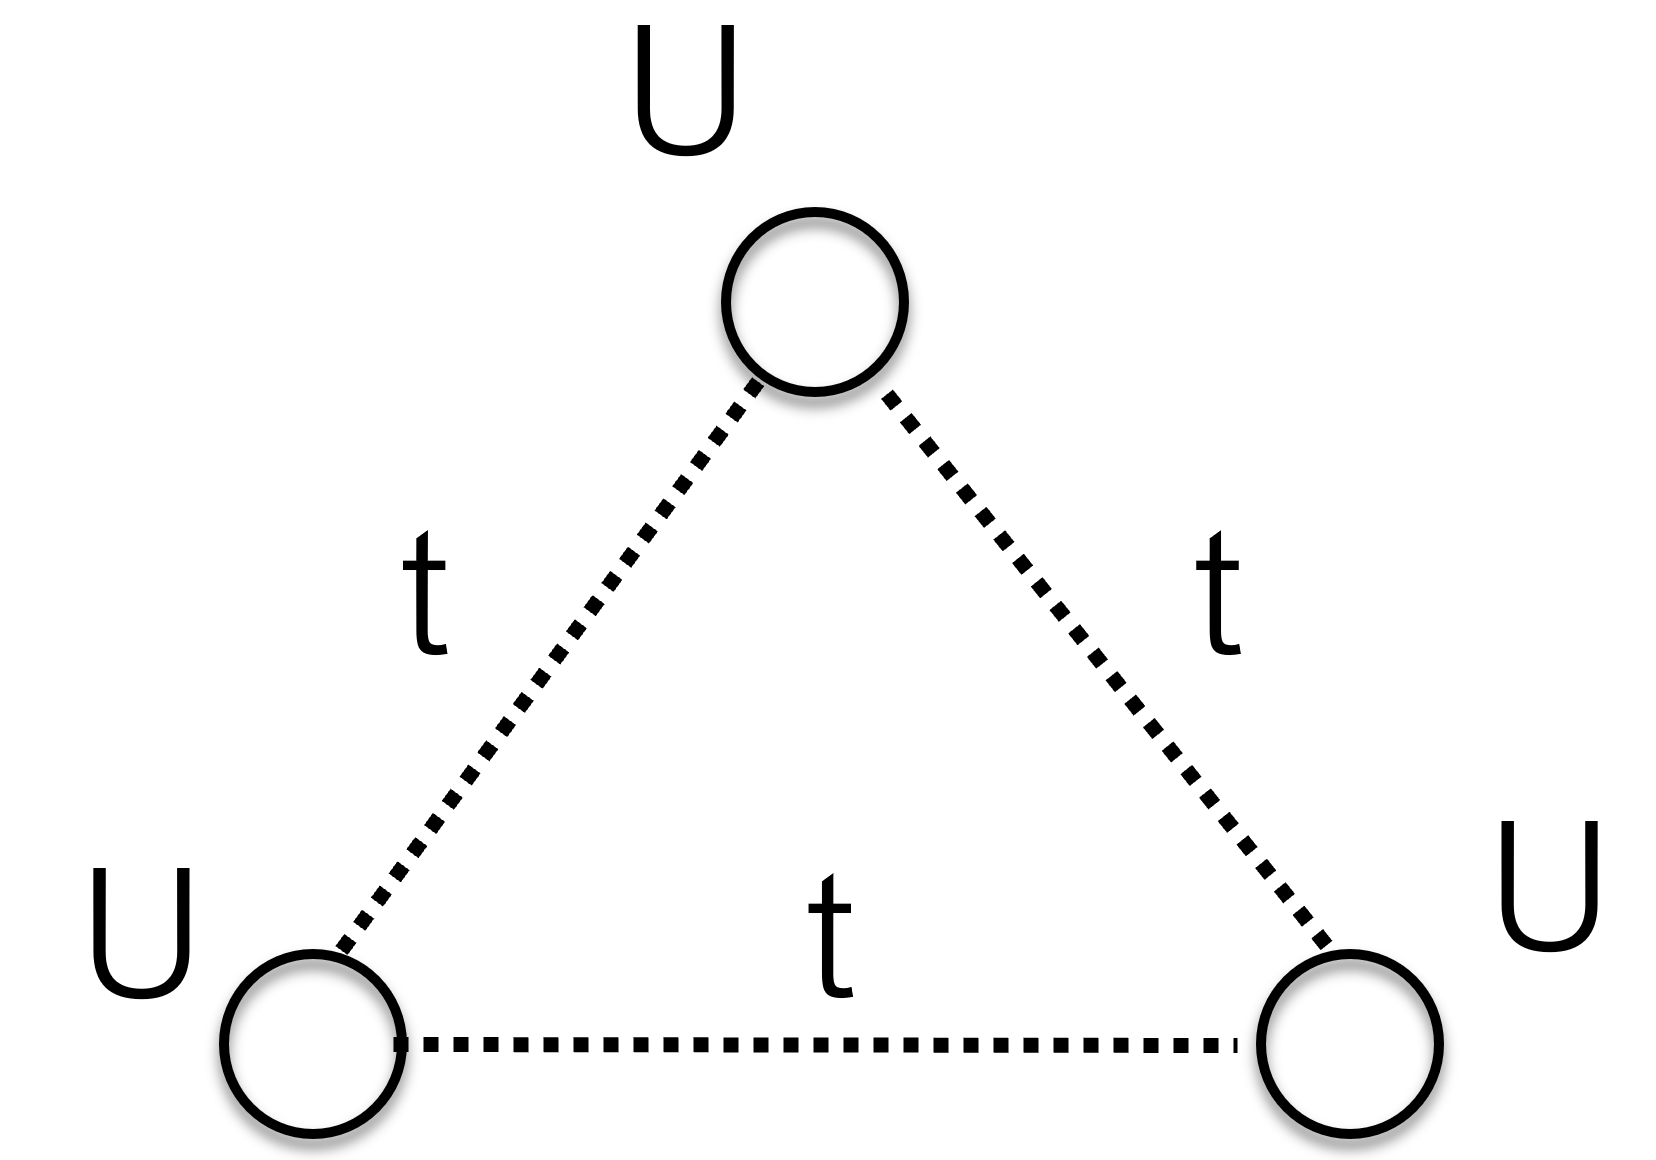
\includegraphics[width=0.4\linewidth]{Hubbard_triangle.png}
	%\caption{Hubbard triangle}
	\label{fig:hubbardtriangle}
\end{figure}	
\end{frame}

\begin{frame}\frametitle{Problem}
Hamiltonian:
	\begin{align}
		H = t \sum_{\langle ij \rangle, \, \sigma} c_{i \sigma}^\dagger c_{j \sigma}^{} + U \sum_{i} n_{i \uparrow} n_{i \downarrow}
	\end{align}

Spin-Spin correlation function:
	\begin{align}
		S = \dfrac{1}{3} \left( S_{1}^{z}S_{2}^{z}  + S_{2}^{z} S_{3}^{z} + S_{3}^{z} S_{1}^{z}  \right)
	\end{align}

Expectation value of S:
	\begin{align}
		\langle S \rangle_T = \dfrac{1}{Z} \sum \langle X | S | X \rangle \exp \left( - \dfrac{E_x}{T} \right)
	\end{align}

Double occupancy:
	\begin{align}
		d = \dfrac{1}{3} \left( n_{1 \uparrow} n_{1 \downarrow} + n_{2 \uparrow} n_{2 \downarrow} + n_{3 \uparrow} n_{3 \downarrow} \right)	
	\end{align}
\end{frame}

%\begin{frame}\frametitle{Problem}
%	\begin{align}
%		H &= t \sum_{\langle ij \rangle, \, \sigma} c_{i \sigma}^\dagger c_{j \sigma}^{} + U \sum_{i} n_{i \uparrow} n_{i \downarrow} \\
%		S &= \dfrac{1}{3} \left( S_{1}^{z}S_{2}^{z}  + S_{2}^{z} S_{3}^{z} + S_{3}^{z} S_{1}^{z}  \right) \\
%		\langle S \rangle_T &= \dfrac{1}{Z} \sum \langle X | S | X \rangle \exp \left( - \dfrac{E_x}{T} \right) \\
%		d &= \dfrac{1}{3} \left( n_{1 \uparrow} n_{1 \downarrow} + n_{2 \uparrow} n_{2 \downarrow} + n_{3 \uparrow} n_{3 \downarrow} \right)	
%	\end{align}
%\end{frame}

\section{Plots}
\begin{frame}\frametitle{S vs. U}
\begin{center}
		\begin{minipage}[t]{0.44\textwidth}
		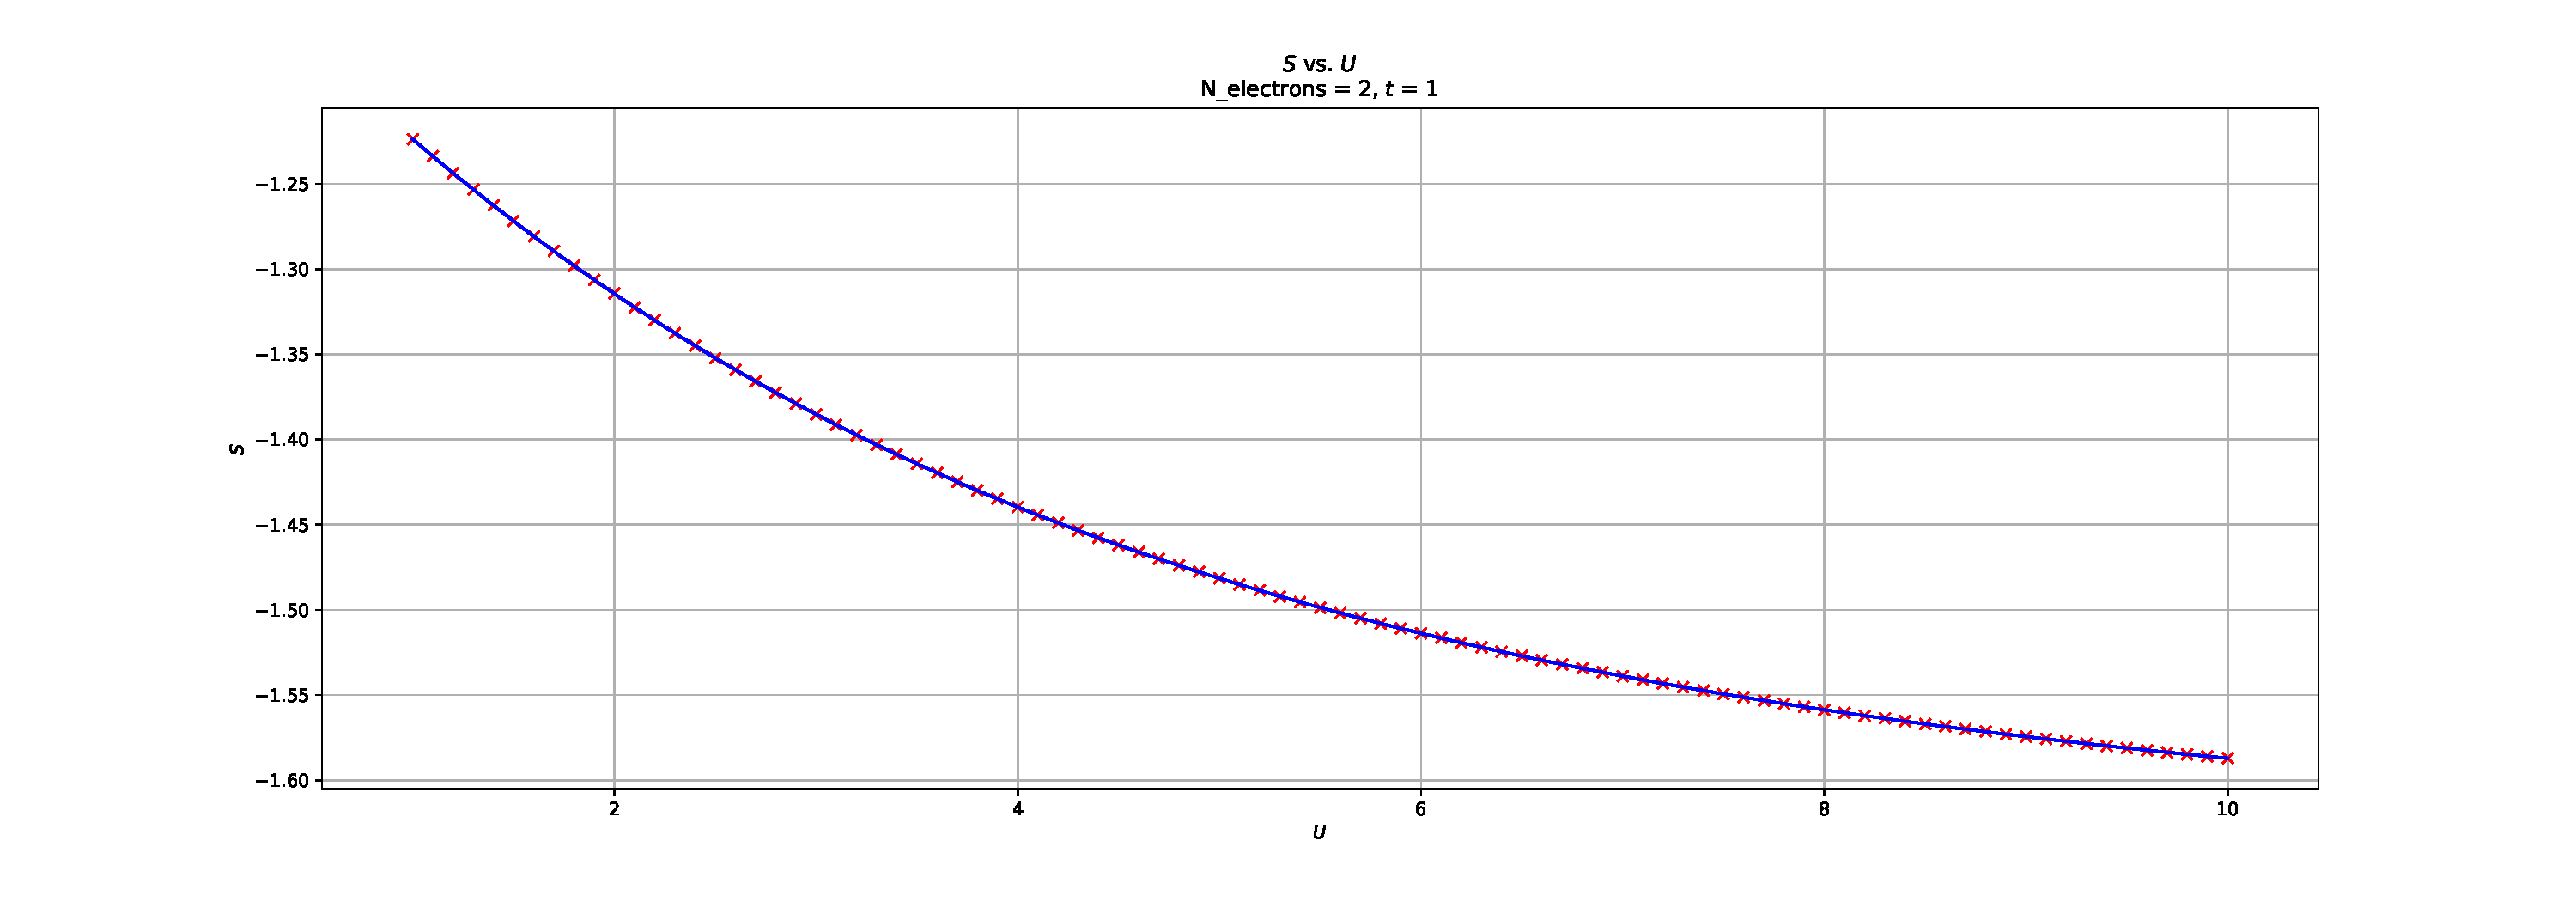
\includegraphics[trim = 5cm 0cm 5cm 0cm, clip, width=1.0\linewidth]{N2_t1/plot_SUi_N2_t1.0.pdf}
	\end{minipage}
	\begin{minipage}[t]{0.44\textwidth}
		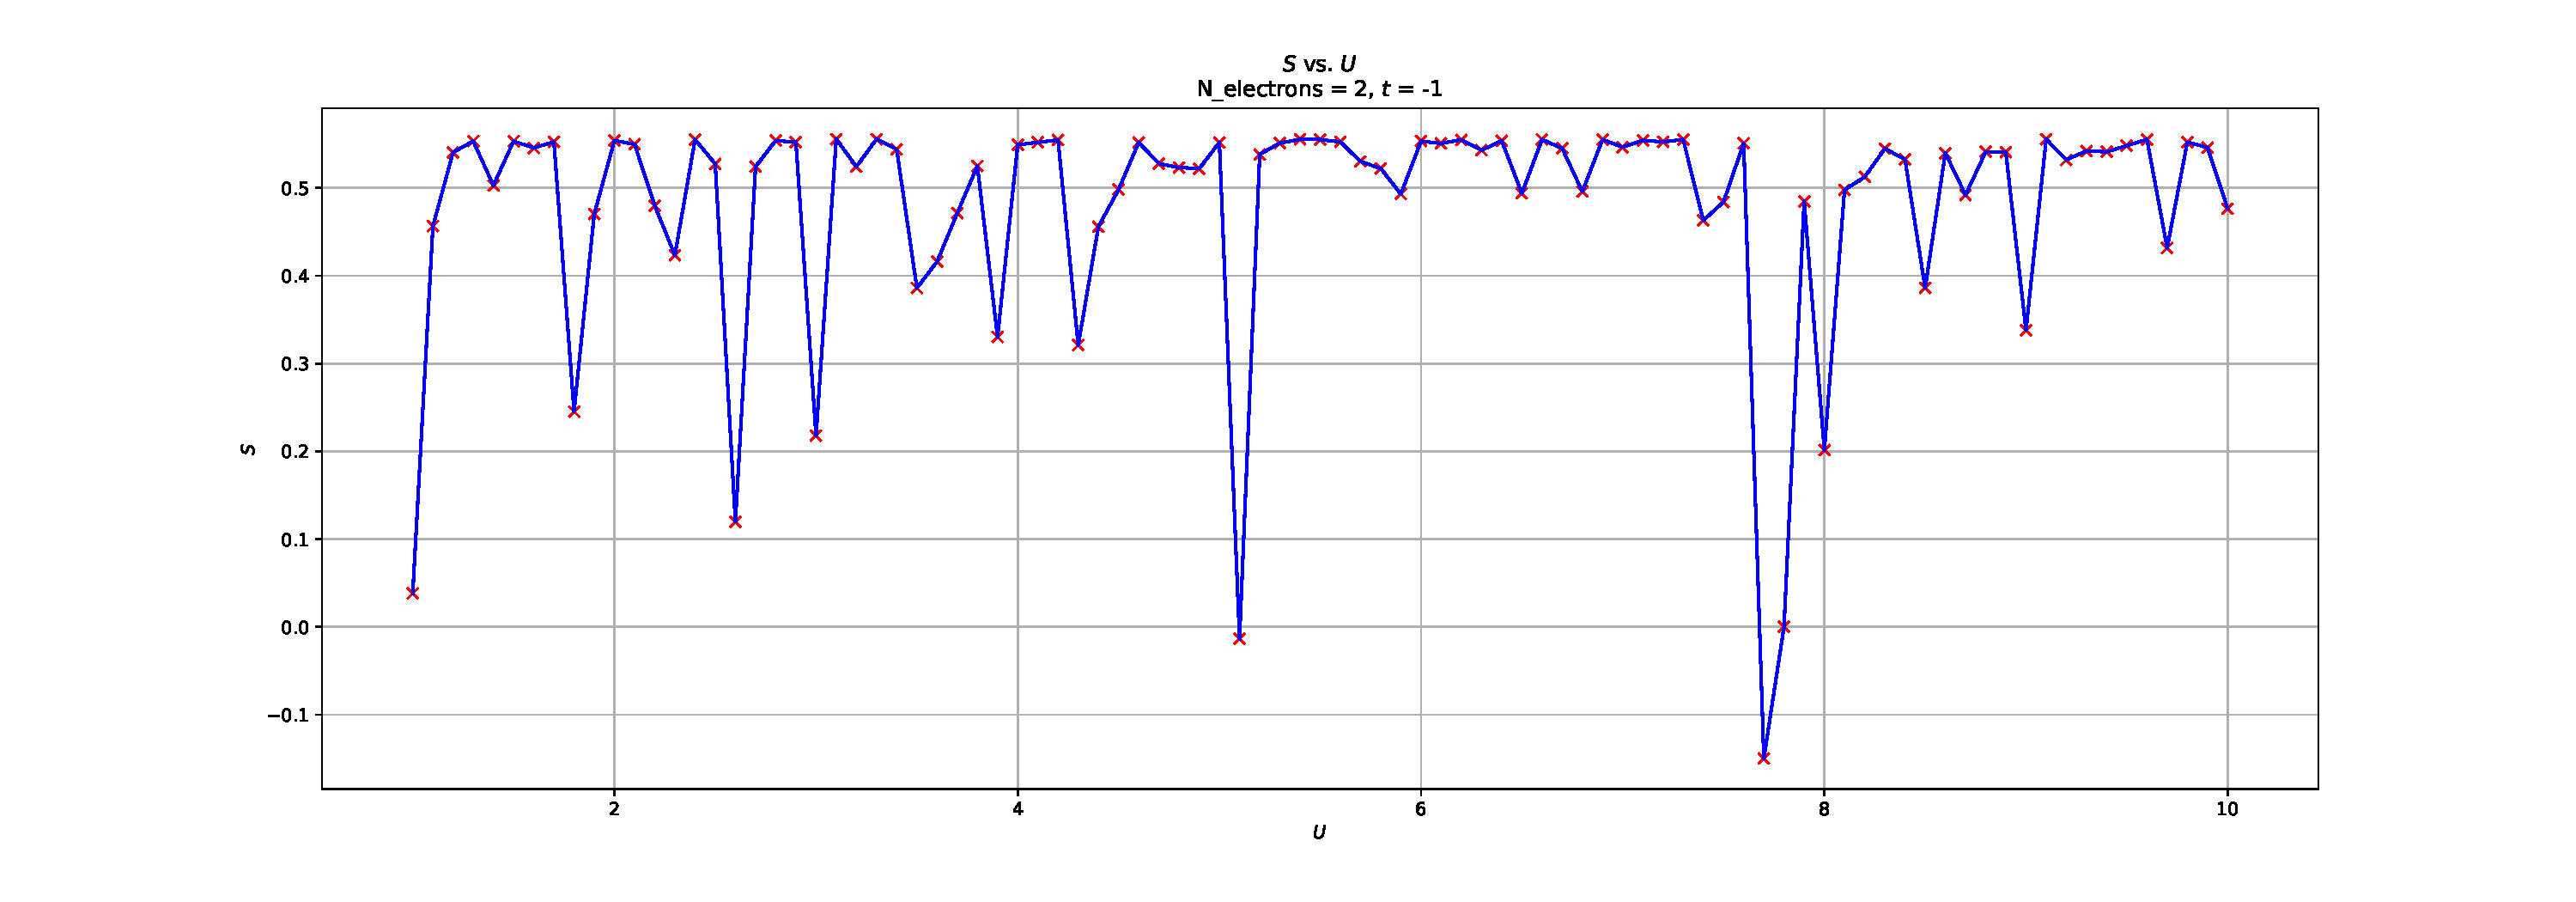
\includegraphics[trim = 5cm 0cm 5cm 0cm, clip, width=1.0\linewidth]{N2_t-1/plot_SUi_N2_t-1.0.pdf}
	\end{minipage}

	\begin{minipage}[t]{0.44\textwidth}
	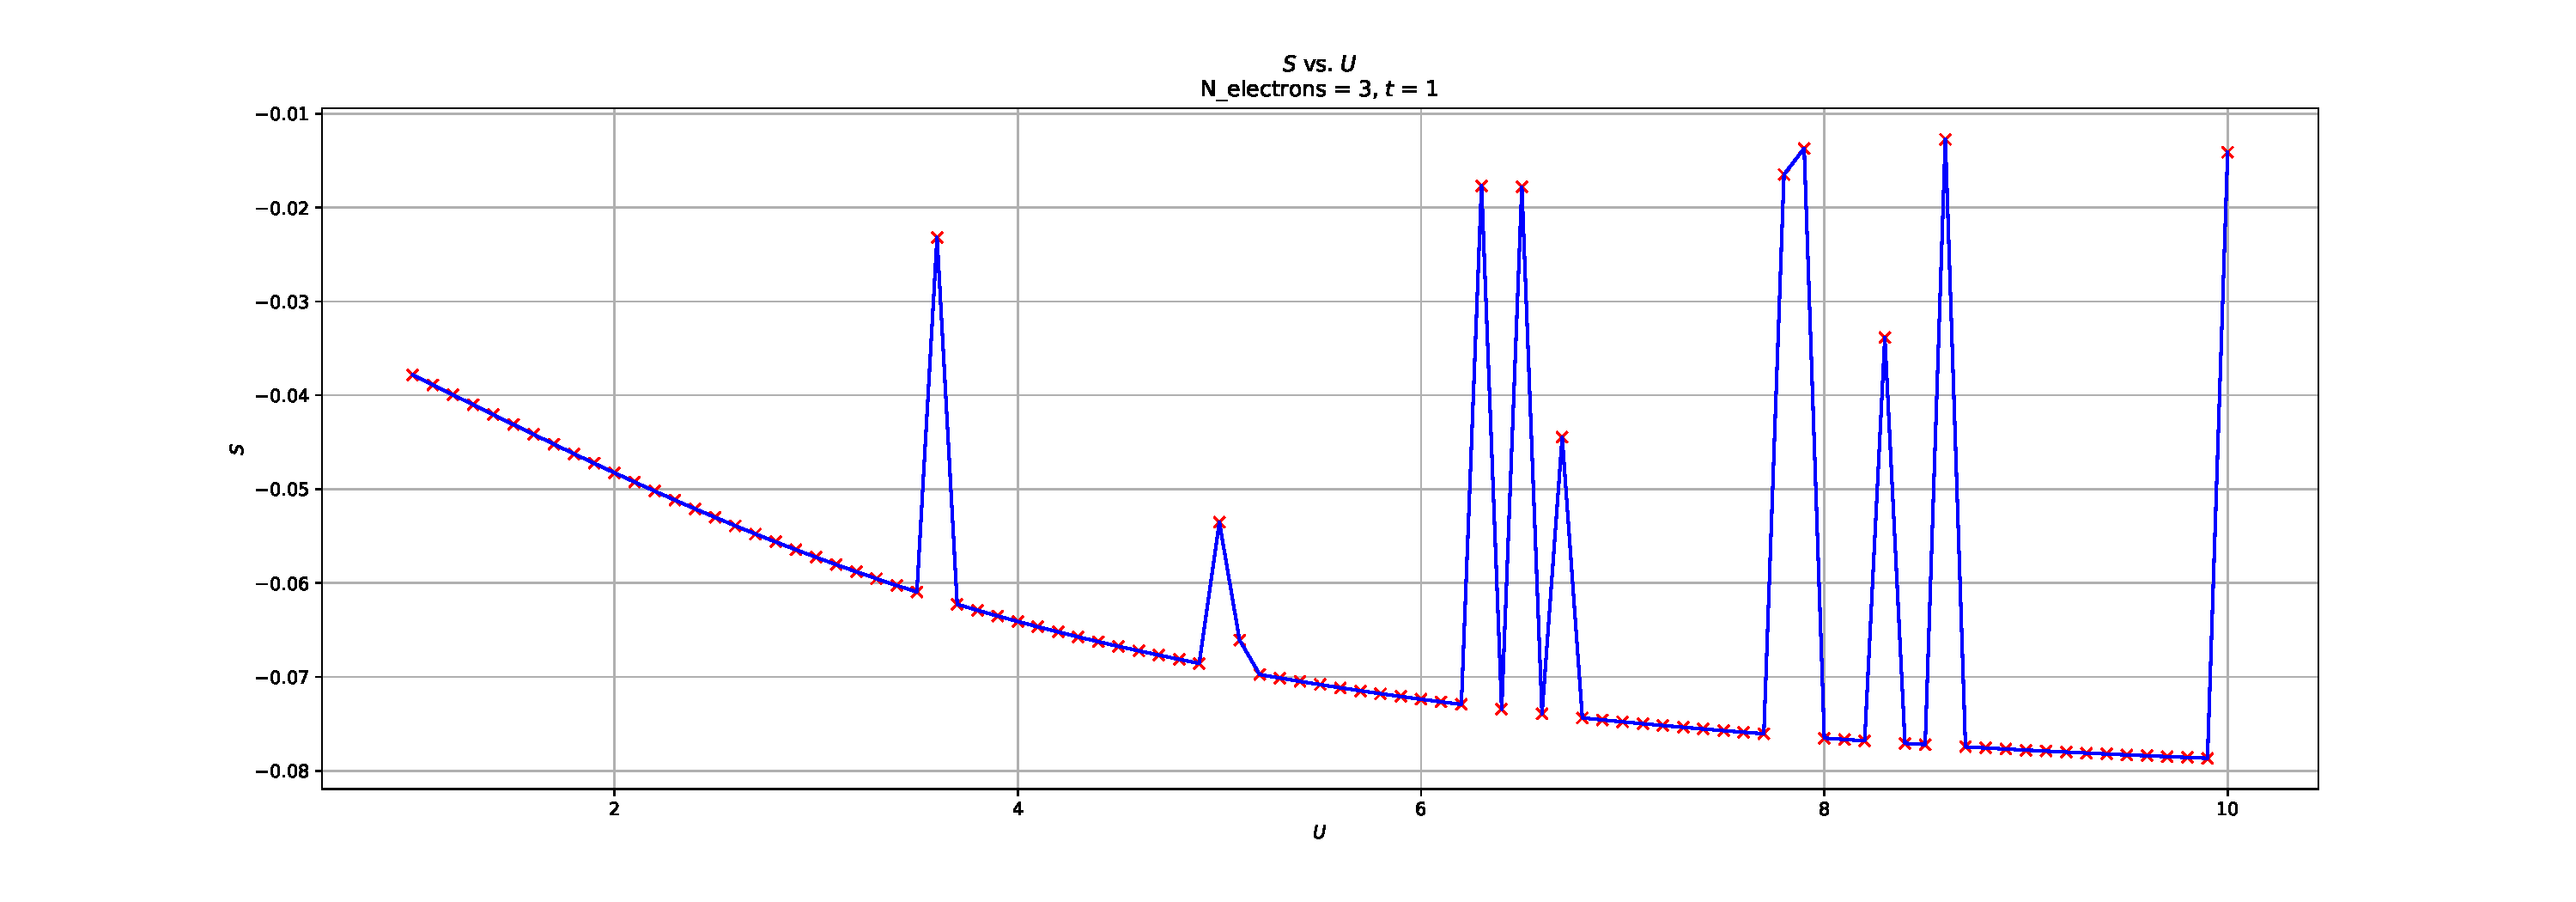
\includegraphics[trim = 5cm 0cm 5cm 0cm, clip, width=1.0\linewidth]{N3_t1/plot_SUi_N3_t1.0.pdf}
	\end{minipage}
	\begin{minipage}[t]{0.44\textwidth}
		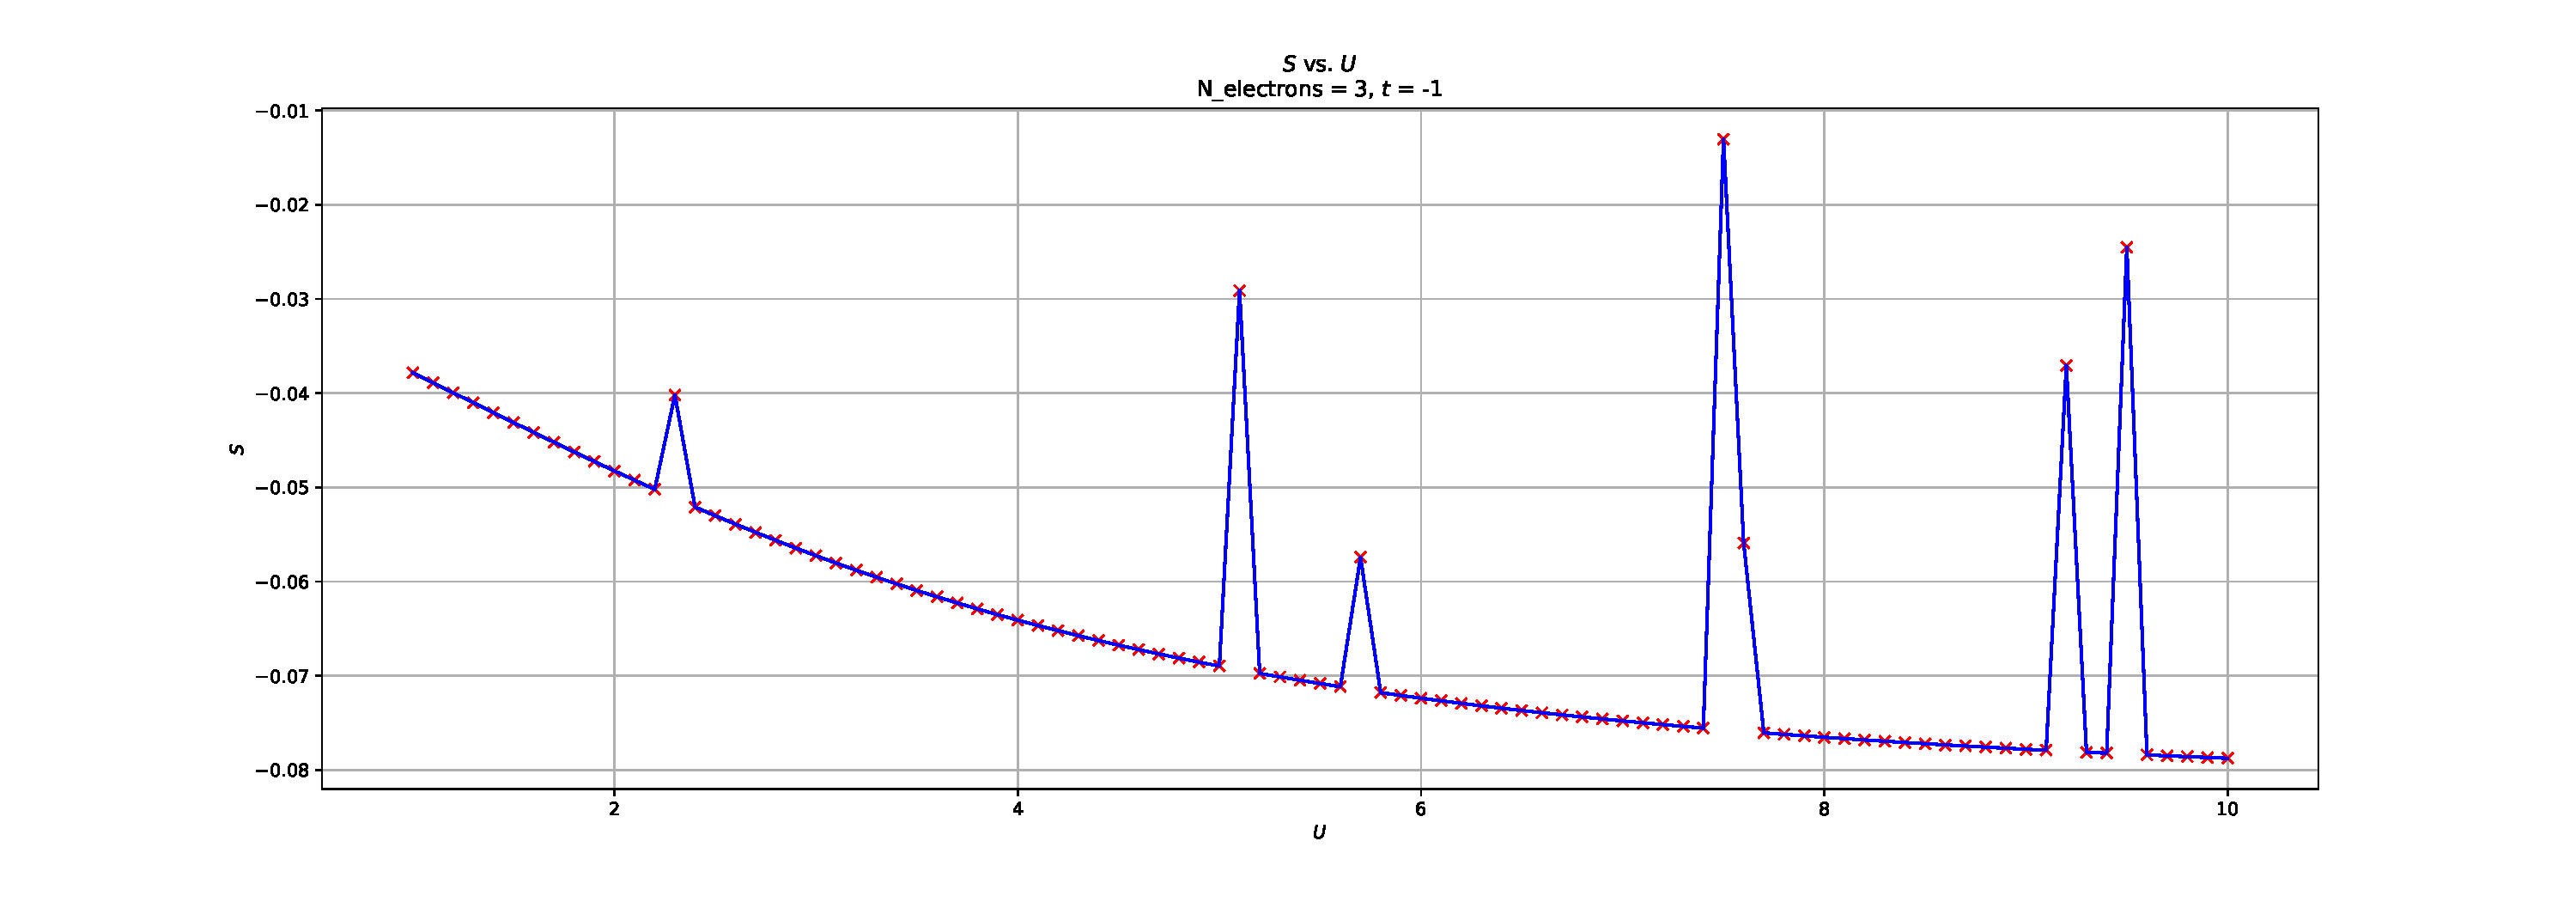
\includegraphics[trim = 5cm 0cm 5cm 0cm, clip, width=1.0\linewidth]{N3_t-1/plot_SUi_N3_t-1.0.pdf}
	\end{minipage}

	\begin{minipage}[t]{0.44\textwidth}
	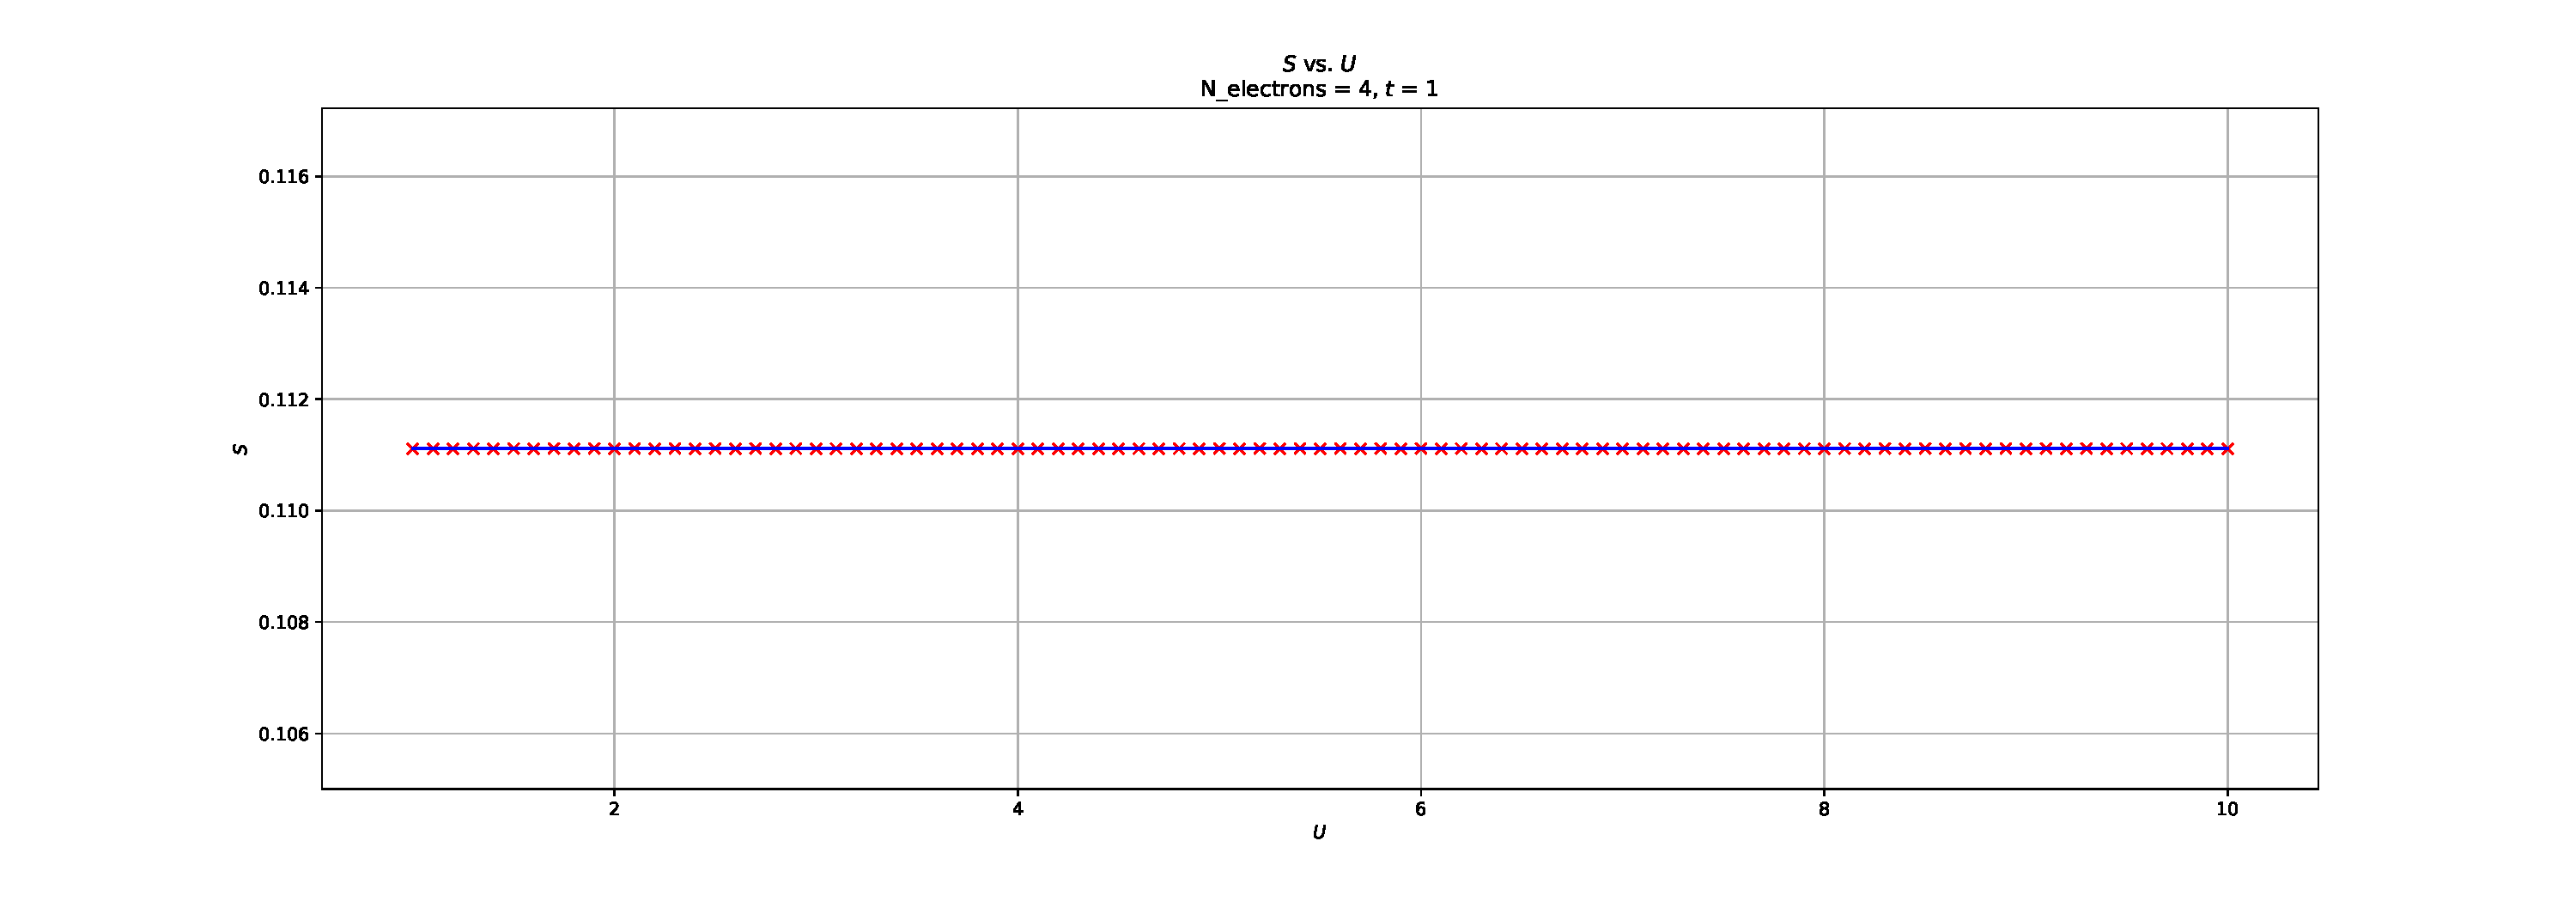
\includegraphics[trim = 5cm 0cm 5cm 0cm, clip, width=1.0\linewidth]{N4_t1/plot_SUi_N4_t1.0.pdf}
	\end{minipage}
	\begin{minipage}[t]{0.44\textwidth}
		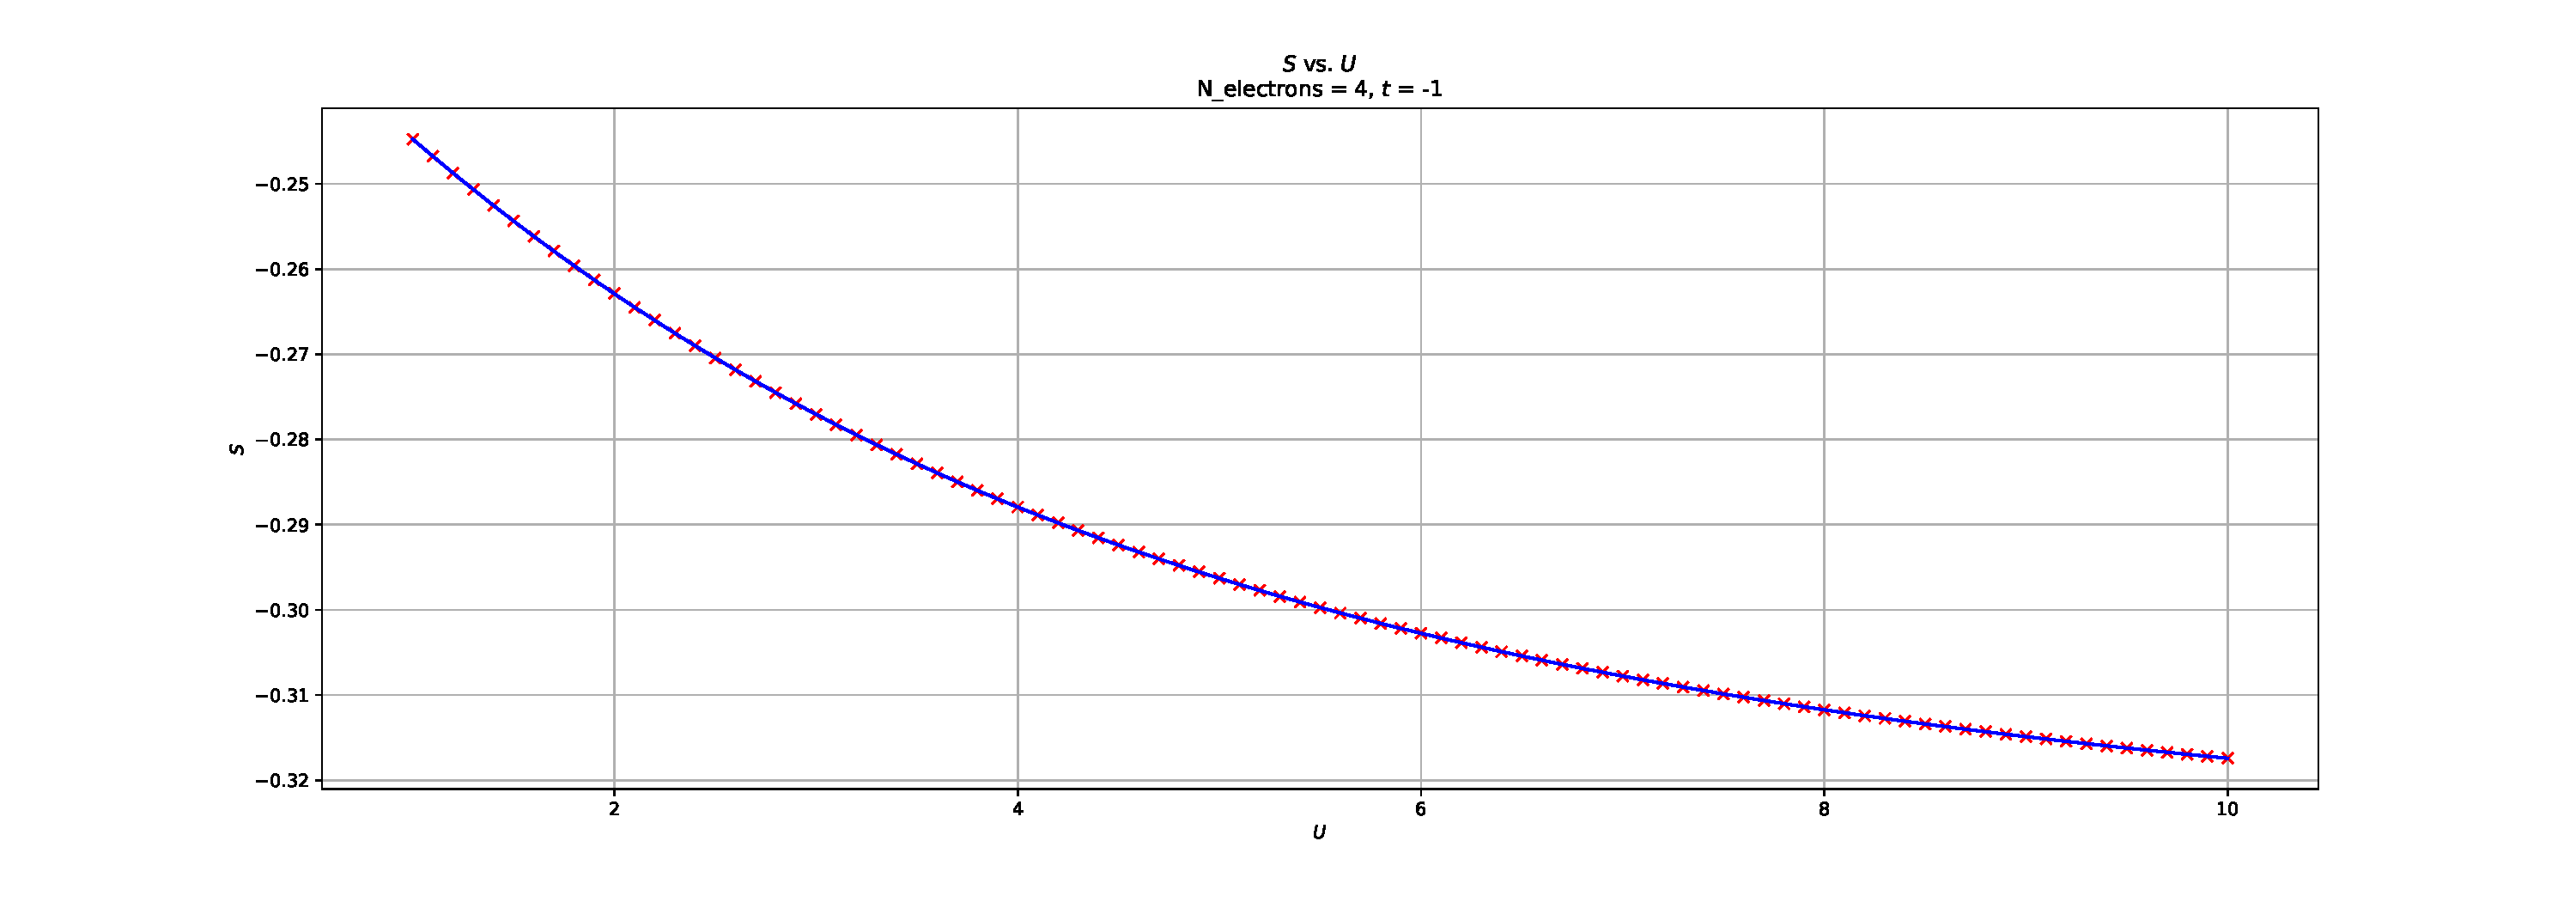
\includegraphics[trim = 5cm 0cm 5cm 0cm, clip, width=1.0\linewidth]{N4_t-1/plot_SUi_N4_t-1.0.pdf}
	\end{minipage}
\end{center}	
\end{frame}

\begin{frame}\frametitle{$\langle$S$\rangle$ vs. T}
	\begin{center}
		\begin{minipage}[t]{0.44\textwidth}
			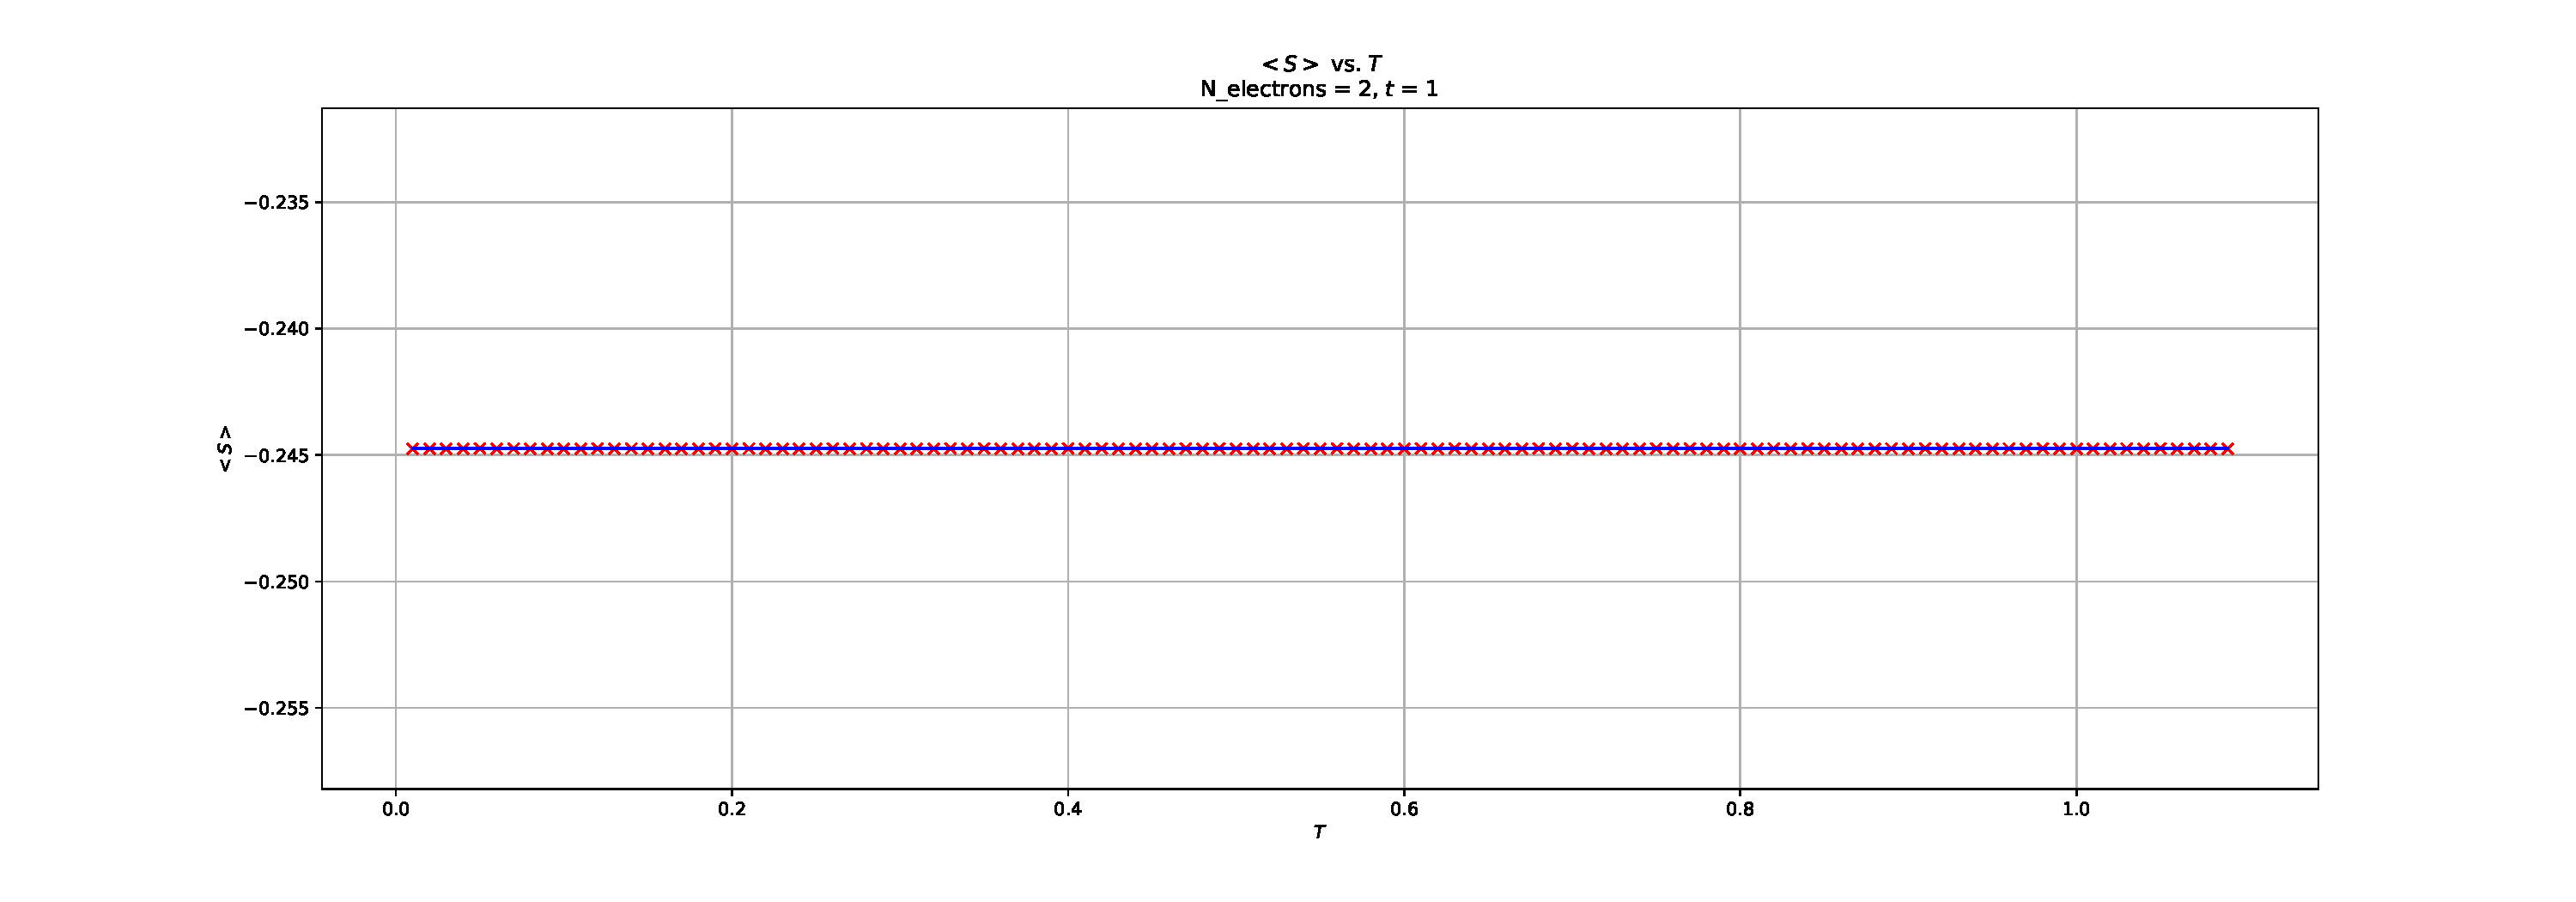
\includegraphics[trim = 5cm 0cm 5cm 0cm, clip, width=1.0\linewidth]{N2_t1/plot_STi_N2_t1.0.pdf}
		\end{minipage}
		\begin{minipage}[t]{0.44\textwidth}
			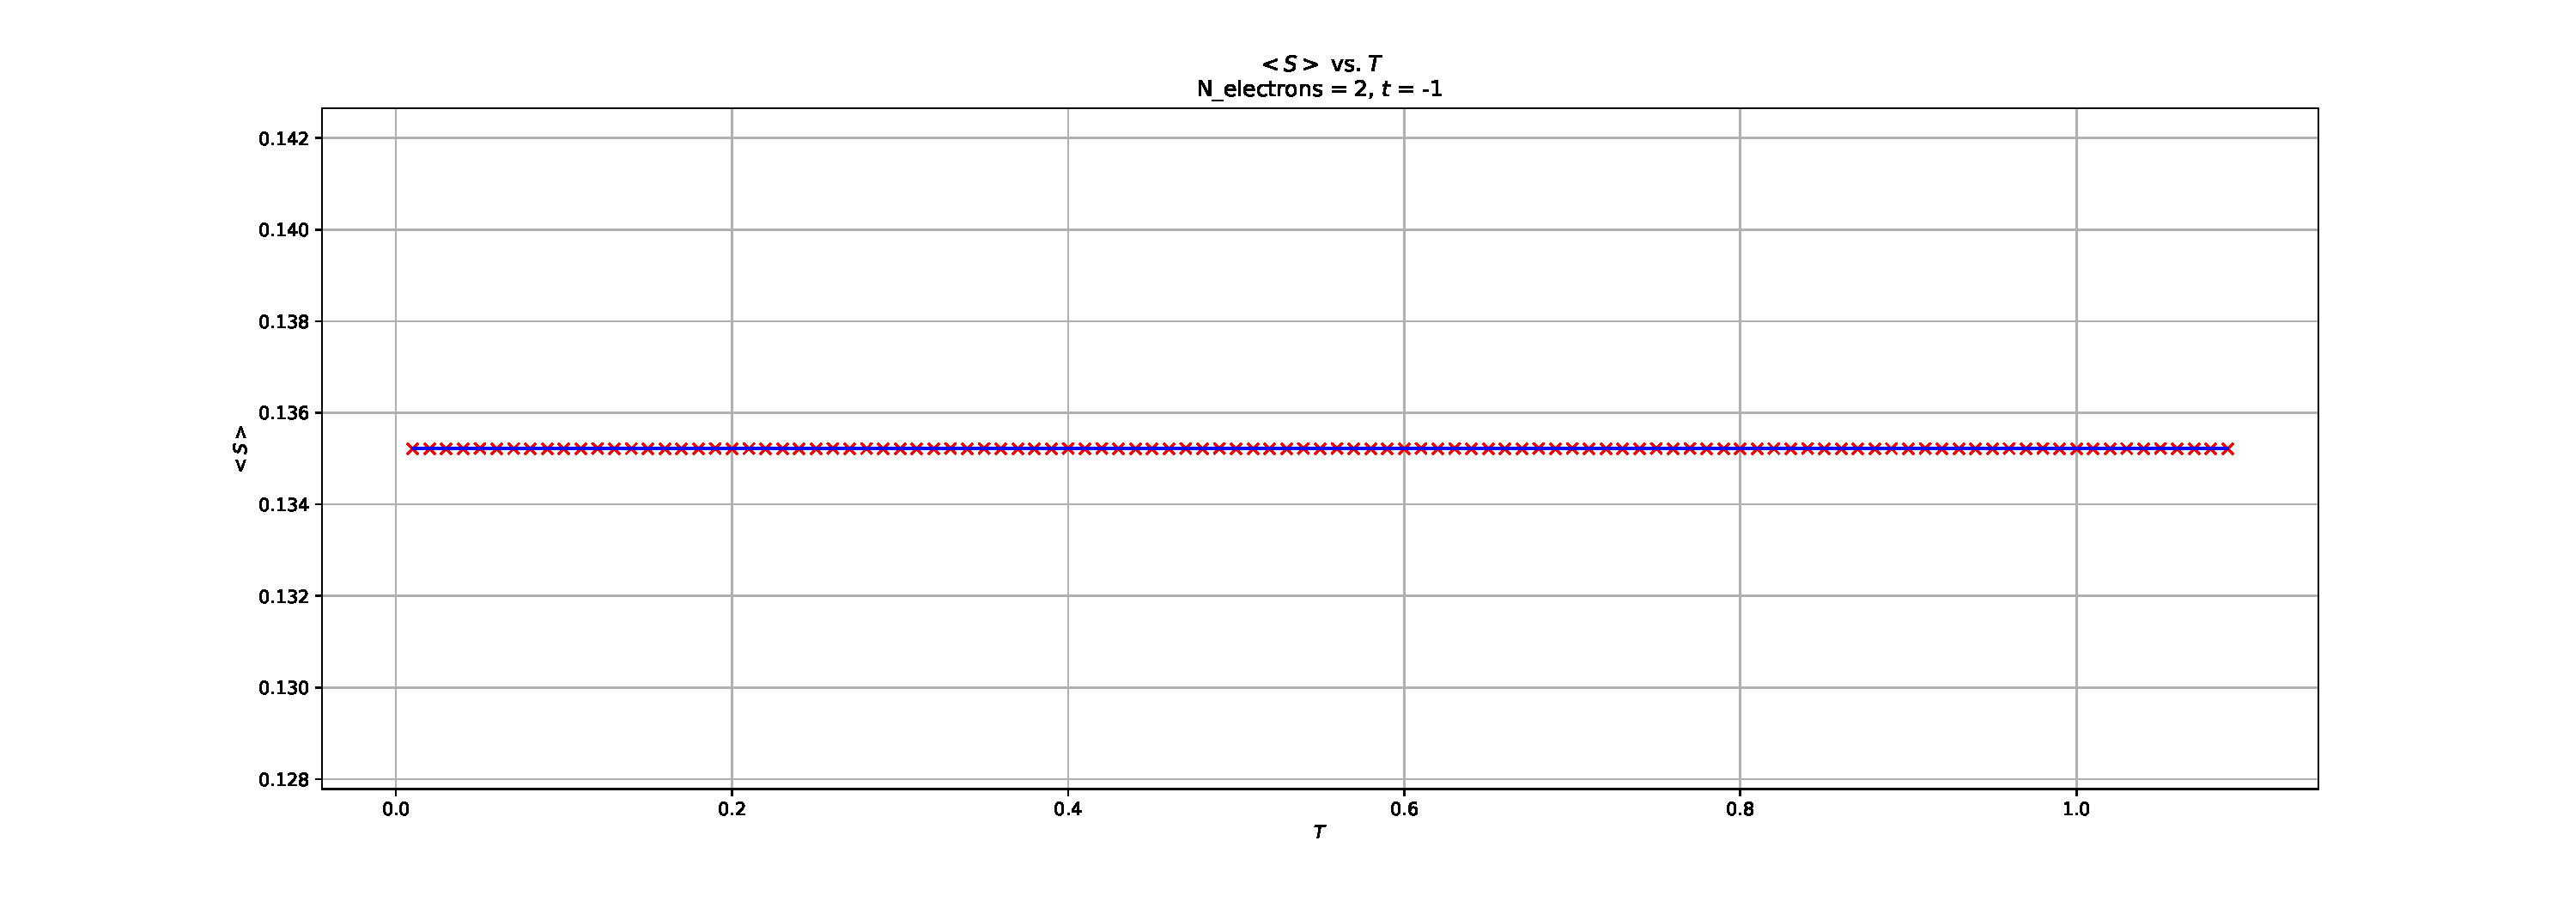
\includegraphics[trim = 5cm 0cm 5cm 0cm, clip, width=1.0\linewidth]{N2_t-1/plot_STi_N2_t-1.0.pdf}
		\end{minipage}
		
		\begin{minipage}[t]{0.44\textwidth}
			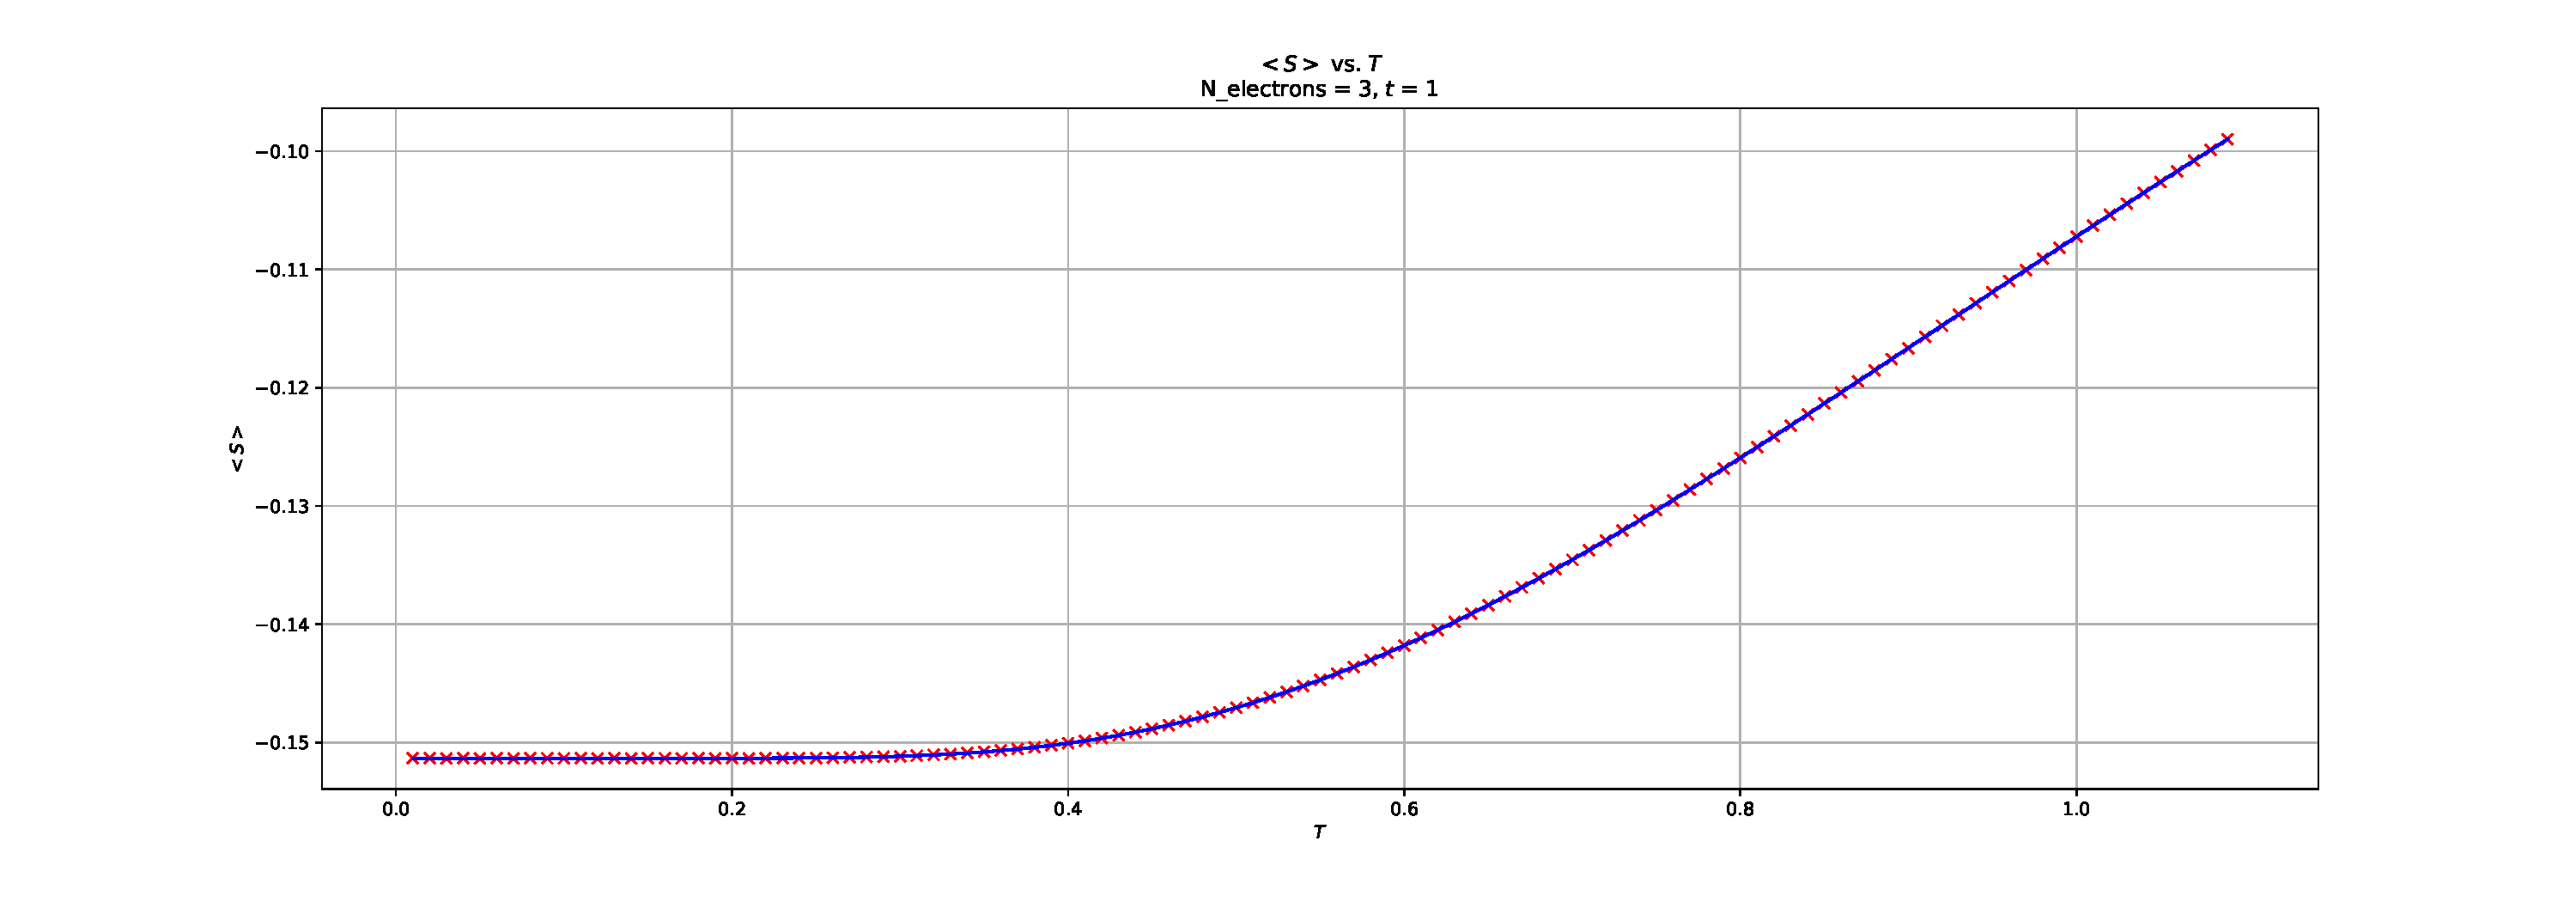
\includegraphics[trim = 5cm 0cm 5cm 0cm, clip, width=1.0\linewidth]{N3_t1/plot_STi_N3_t1.0.pdf}
		\end{minipage}
		\begin{minipage}[t]{0.44\textwidth}
			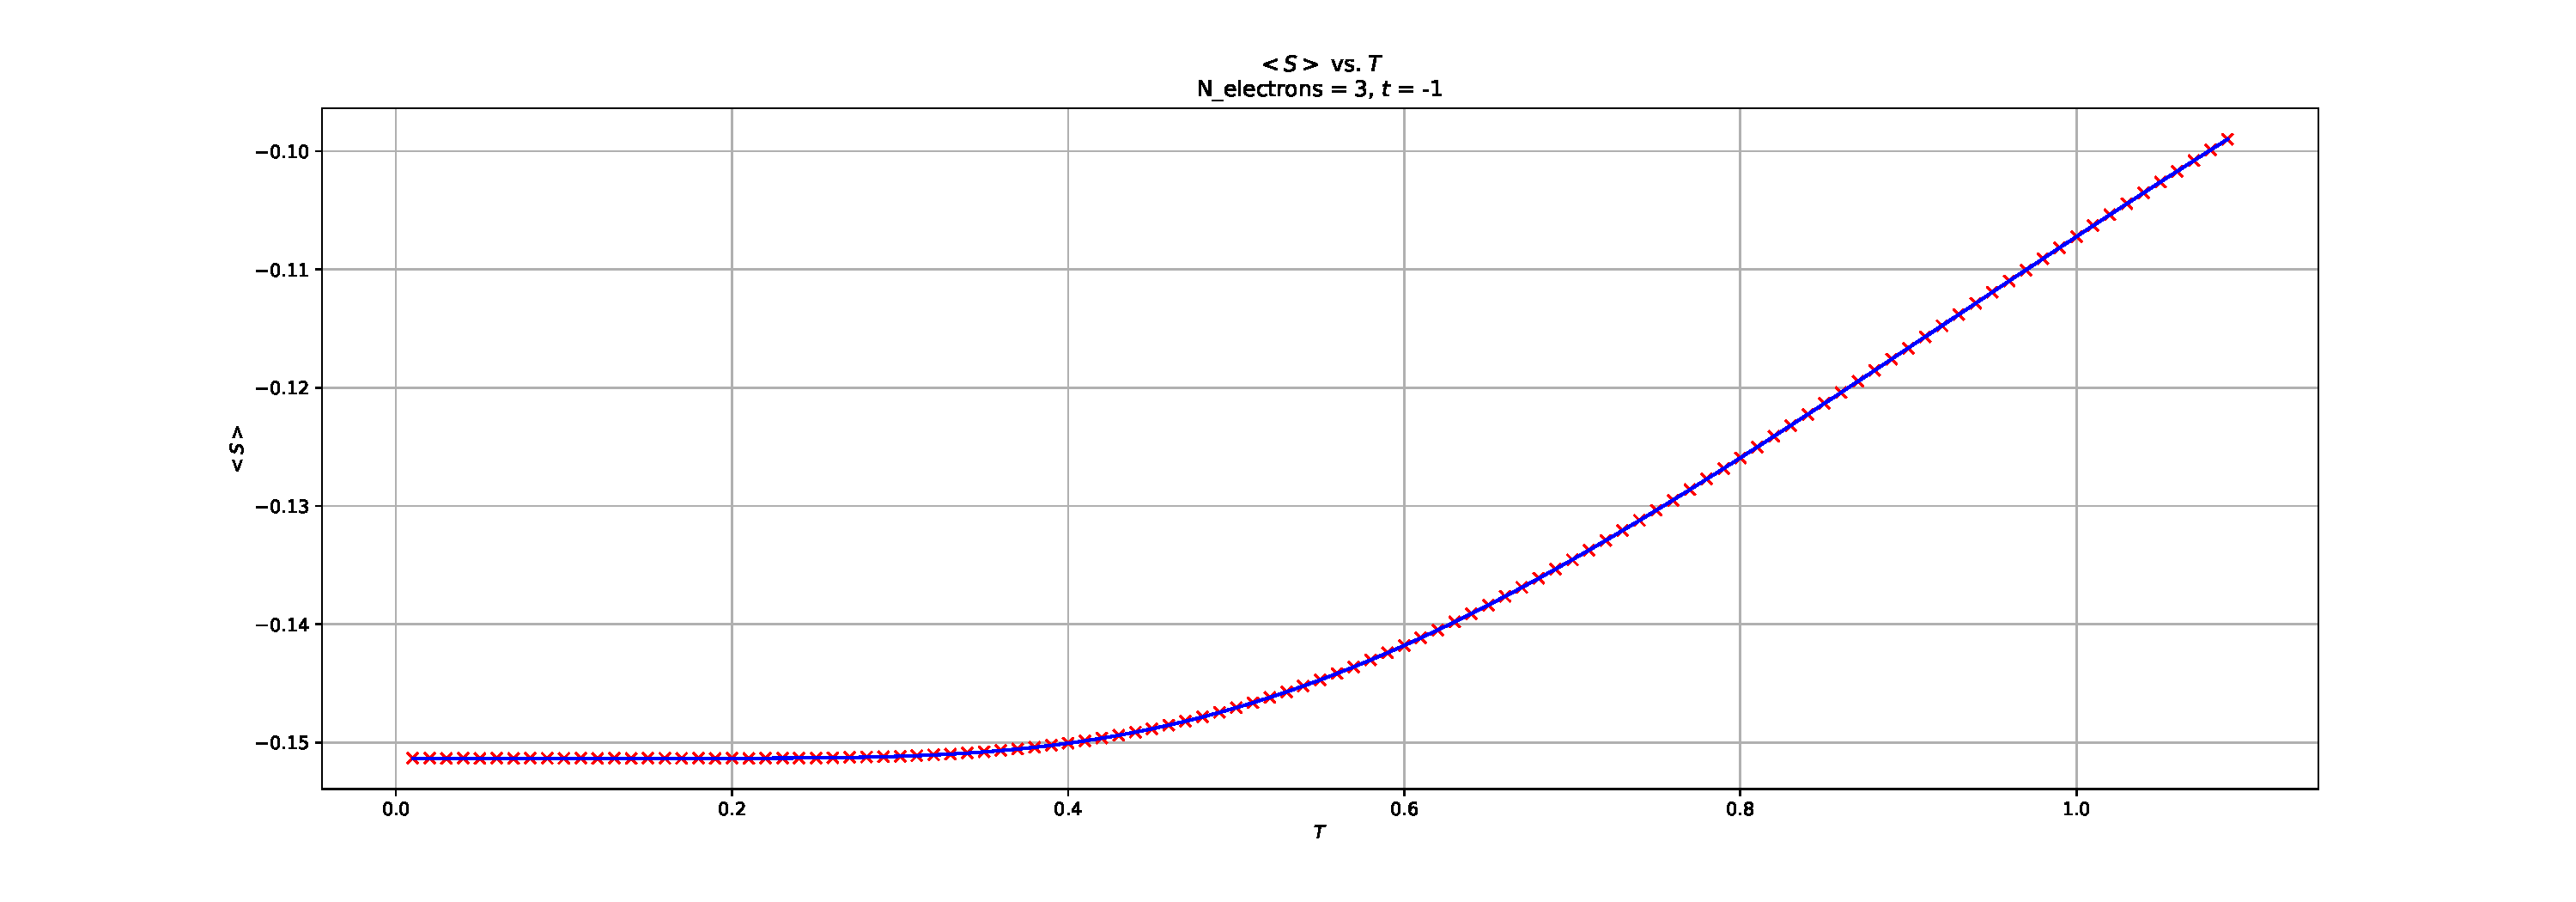
\includegraphics[trim = 5cm 0cm 5cm 0cm, clip, width=1.0\linewidth]{N3_t-1/plot_STi_N3_t-1.0.pdf}
		\end{minipage}
		
		\begin{minipage}[t]{0.44\textwidth}
			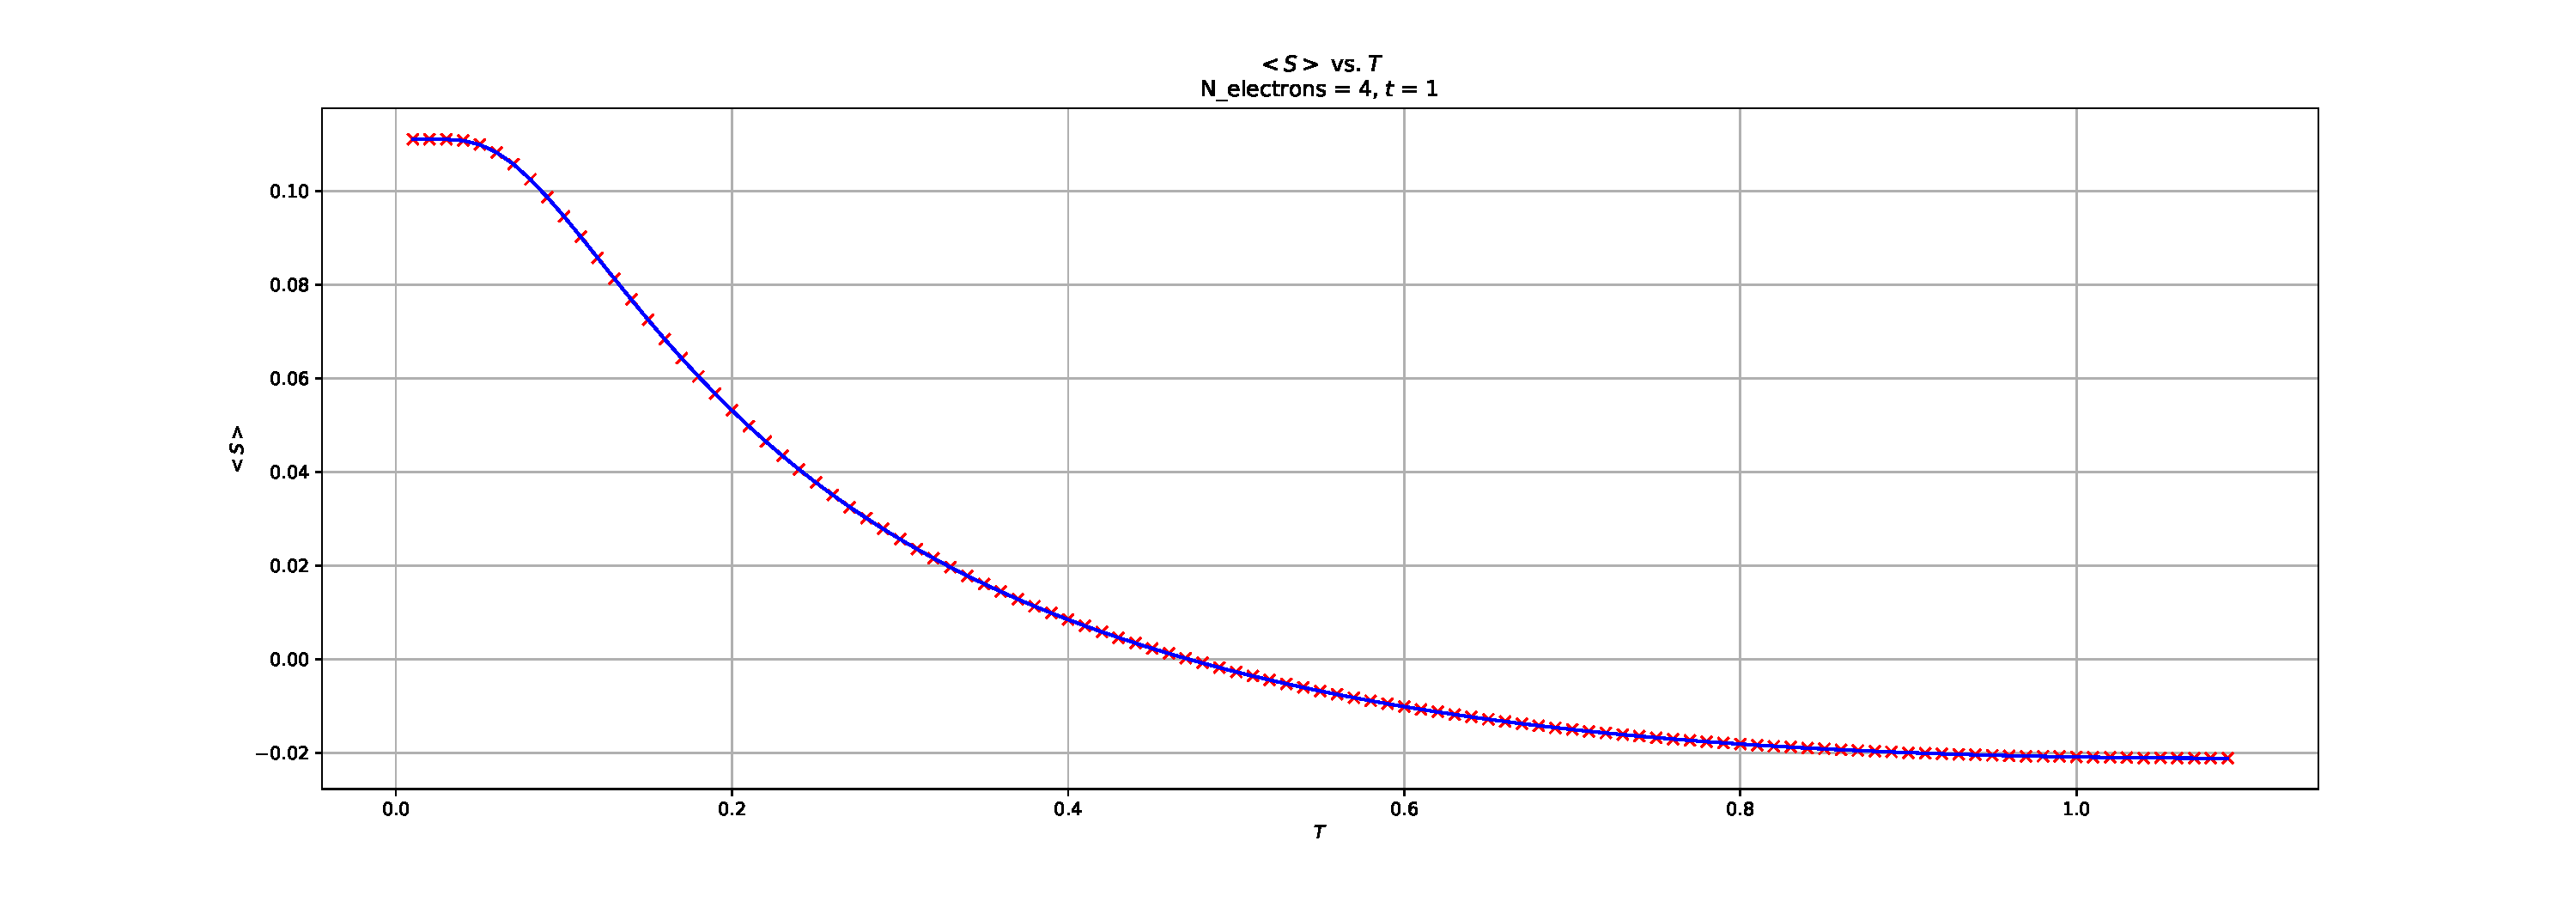
\includegraphics[trim = 5cm 0cm 5cm 0cm, clip, width=1.0\linewidth]{N4_t1/plot_STi_N4_t1.0.pdf}
		\end{minipage}
		\begin{minipage}[t]{0.44\textwidth}
			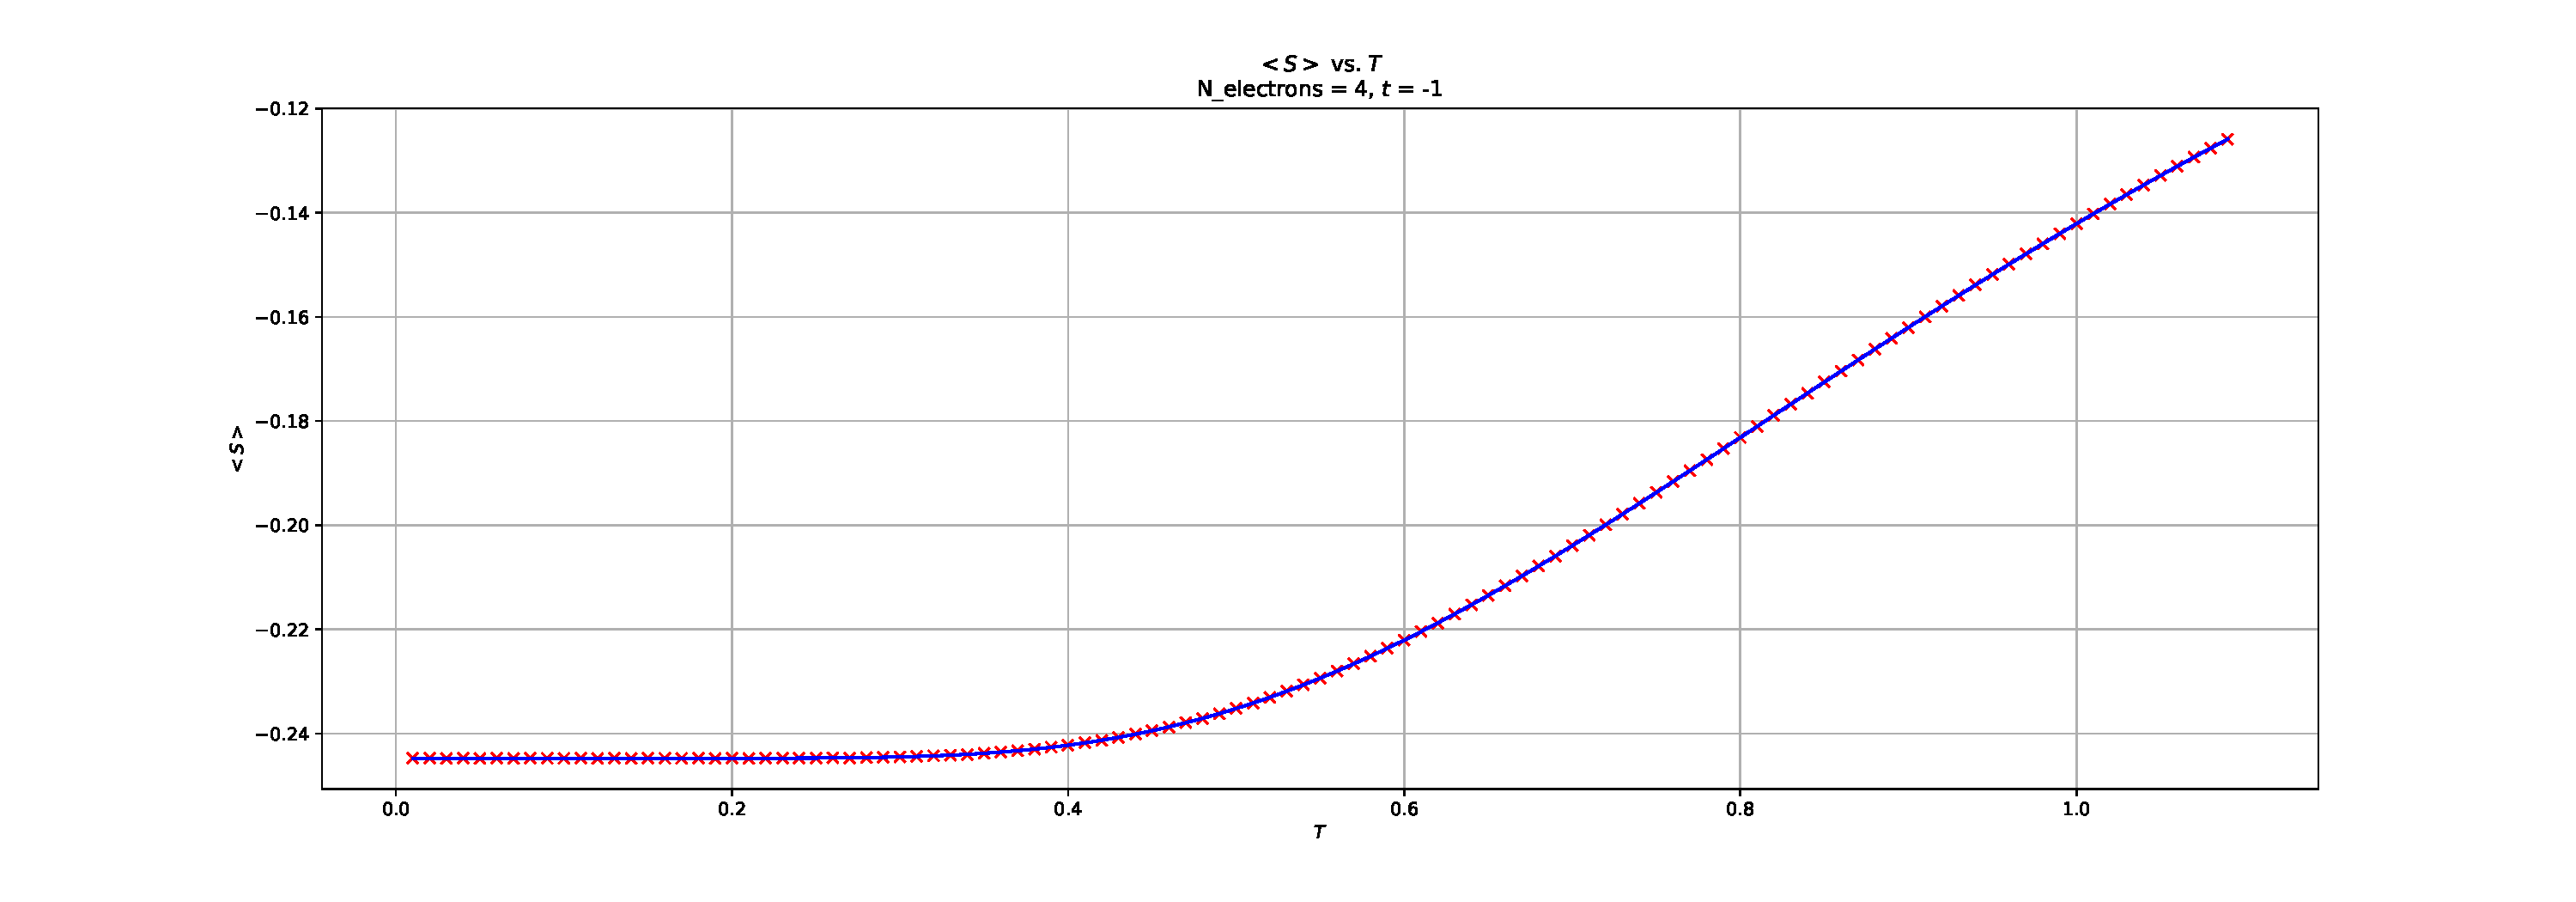
\includegraphics[trim = 5cm 0cm 5cm 0cm, clip, width=1.0\linewidth]{N4_t-1/plot_STi_N4_t-1.0.pdf}
		\end{minipage}
	\end{center}	
\end{frame}

\begin{frame}\frametitle{d vs. U}
	\begin{center}
		\begin{minipage}[t]{0.44\textwidth}
			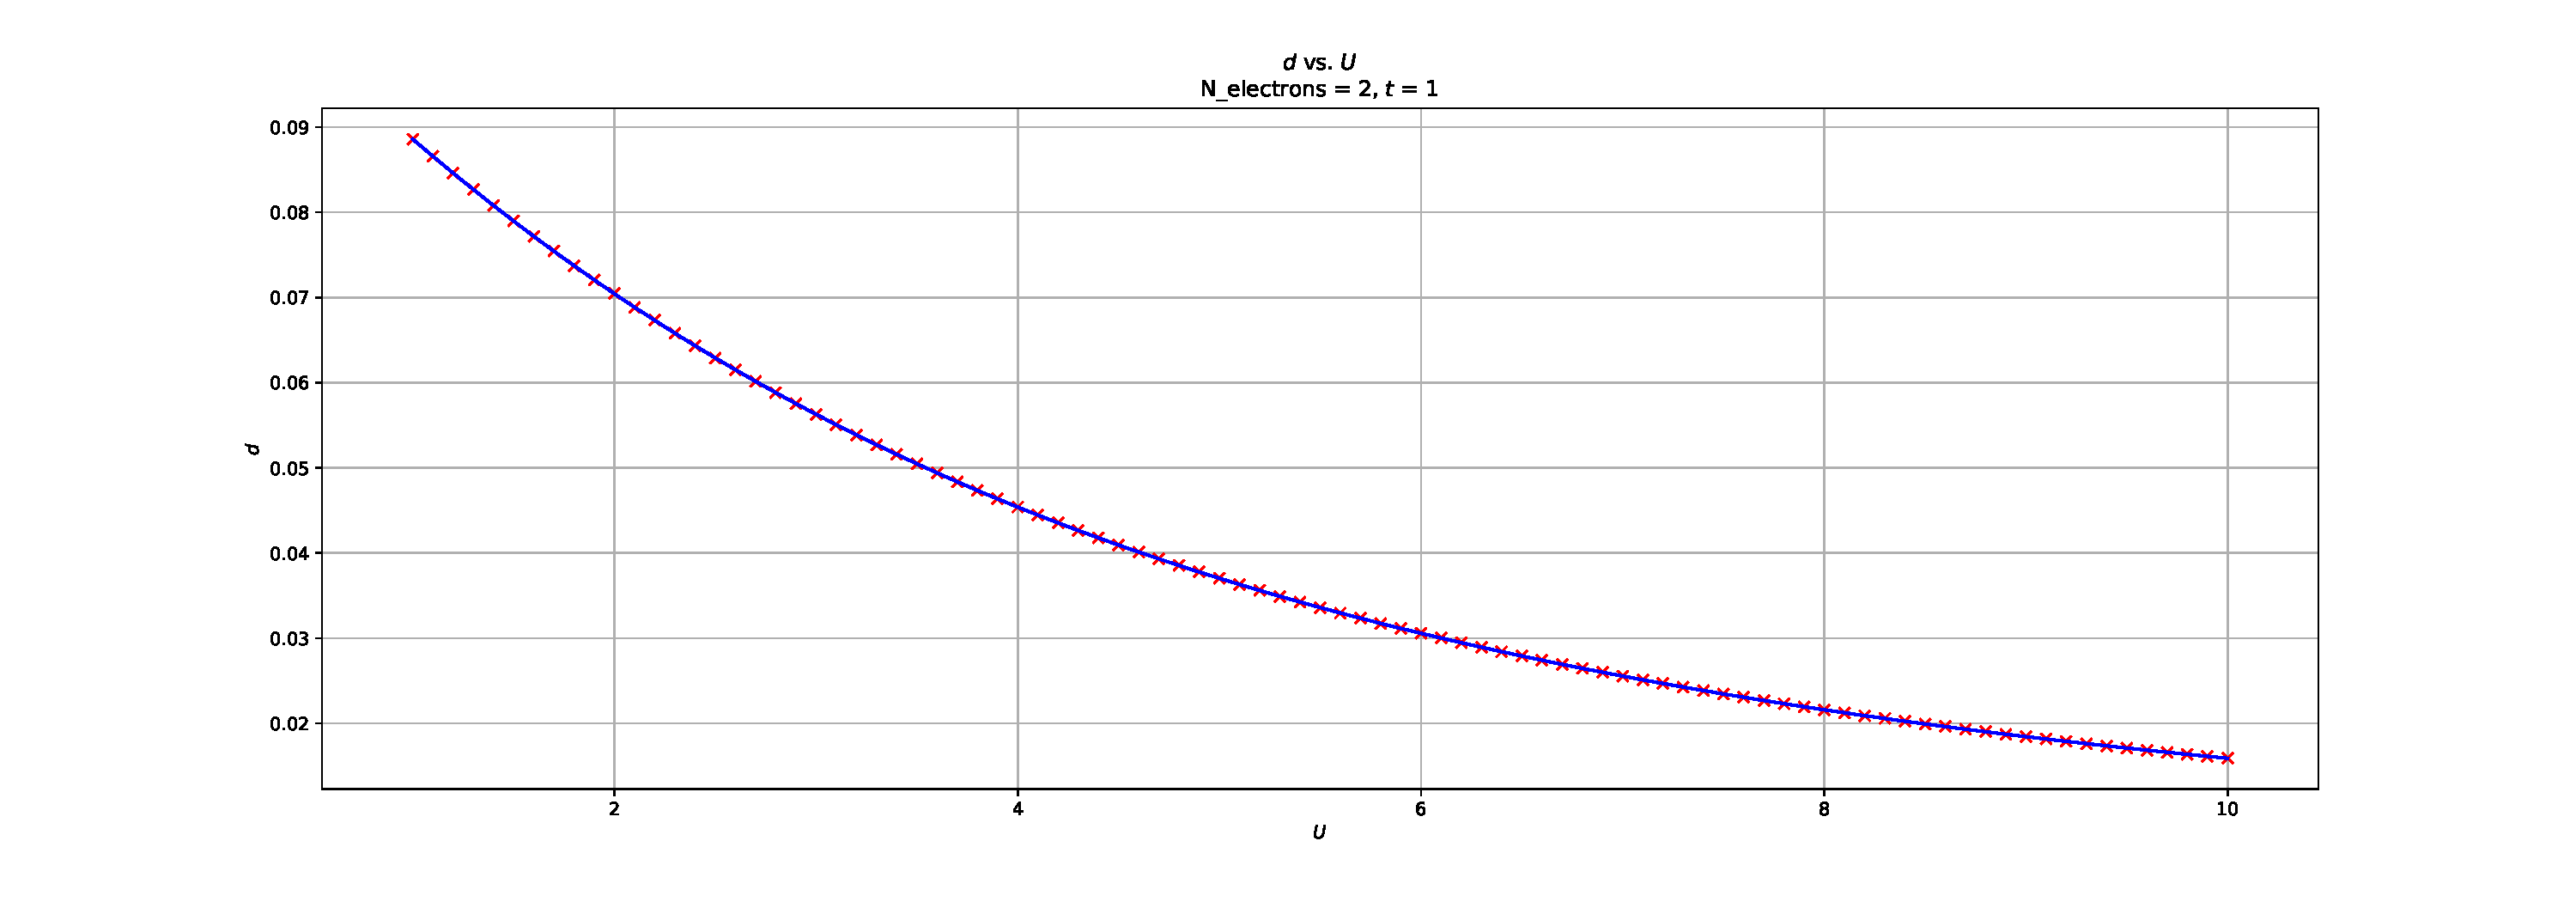
\includegraphics[trim = 5cm 0cm 5cm 0cm, clip, width=1.0\linewidth]{N2_t1/plot_dUi_N2_t1.0.pdf}
		\end{minipage}
		\begin{minipage}[t]{0.44\textwidth}
			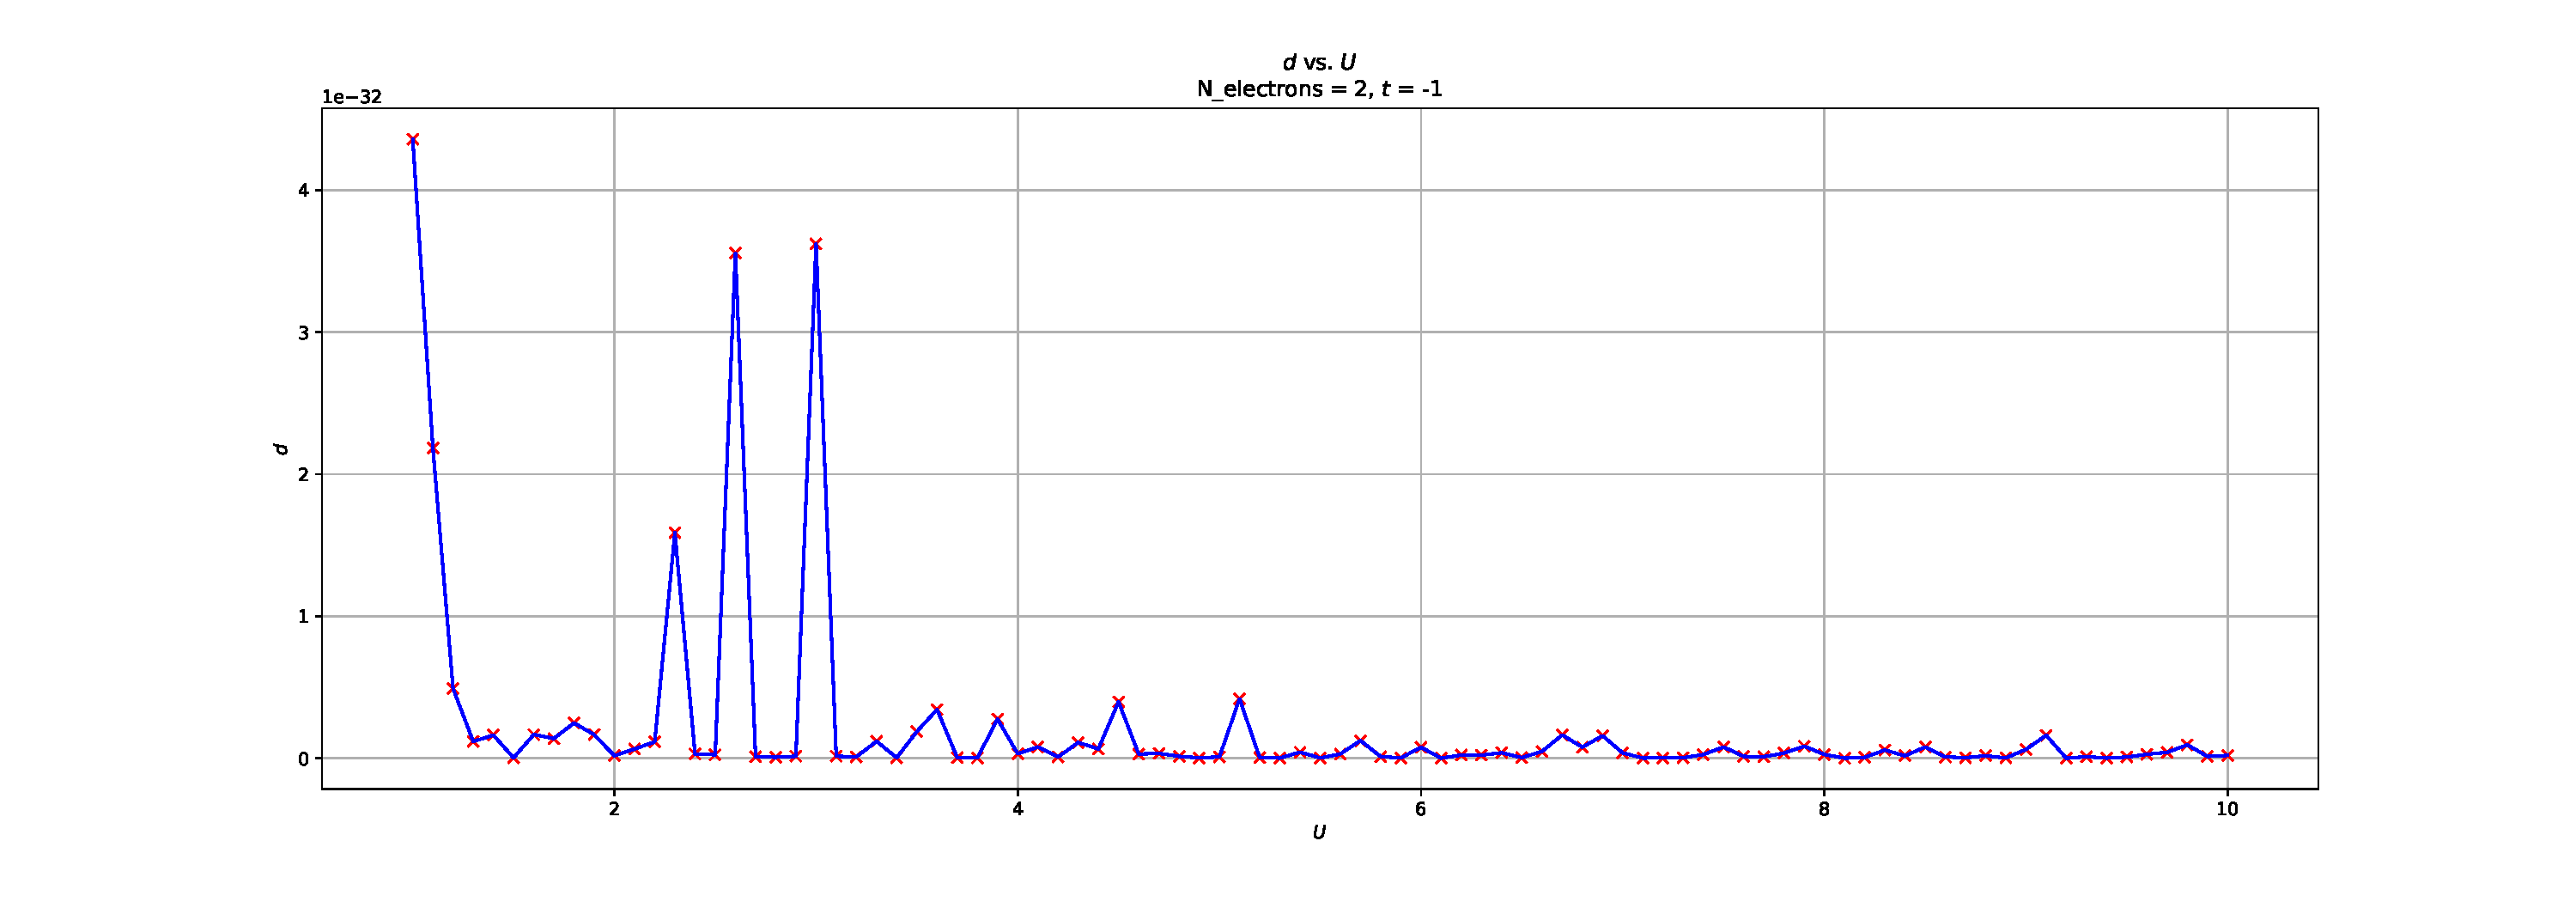
\includegraphics[trim = 5cm 0cm 5cm 0cm, clip, width=1.0\linewidth]{N2_t-1/plot_dUi_N2_t-1.0.pdf}
		\end{minipage}
		
		\begin{minipage}[t]{0.44\textwidth}
			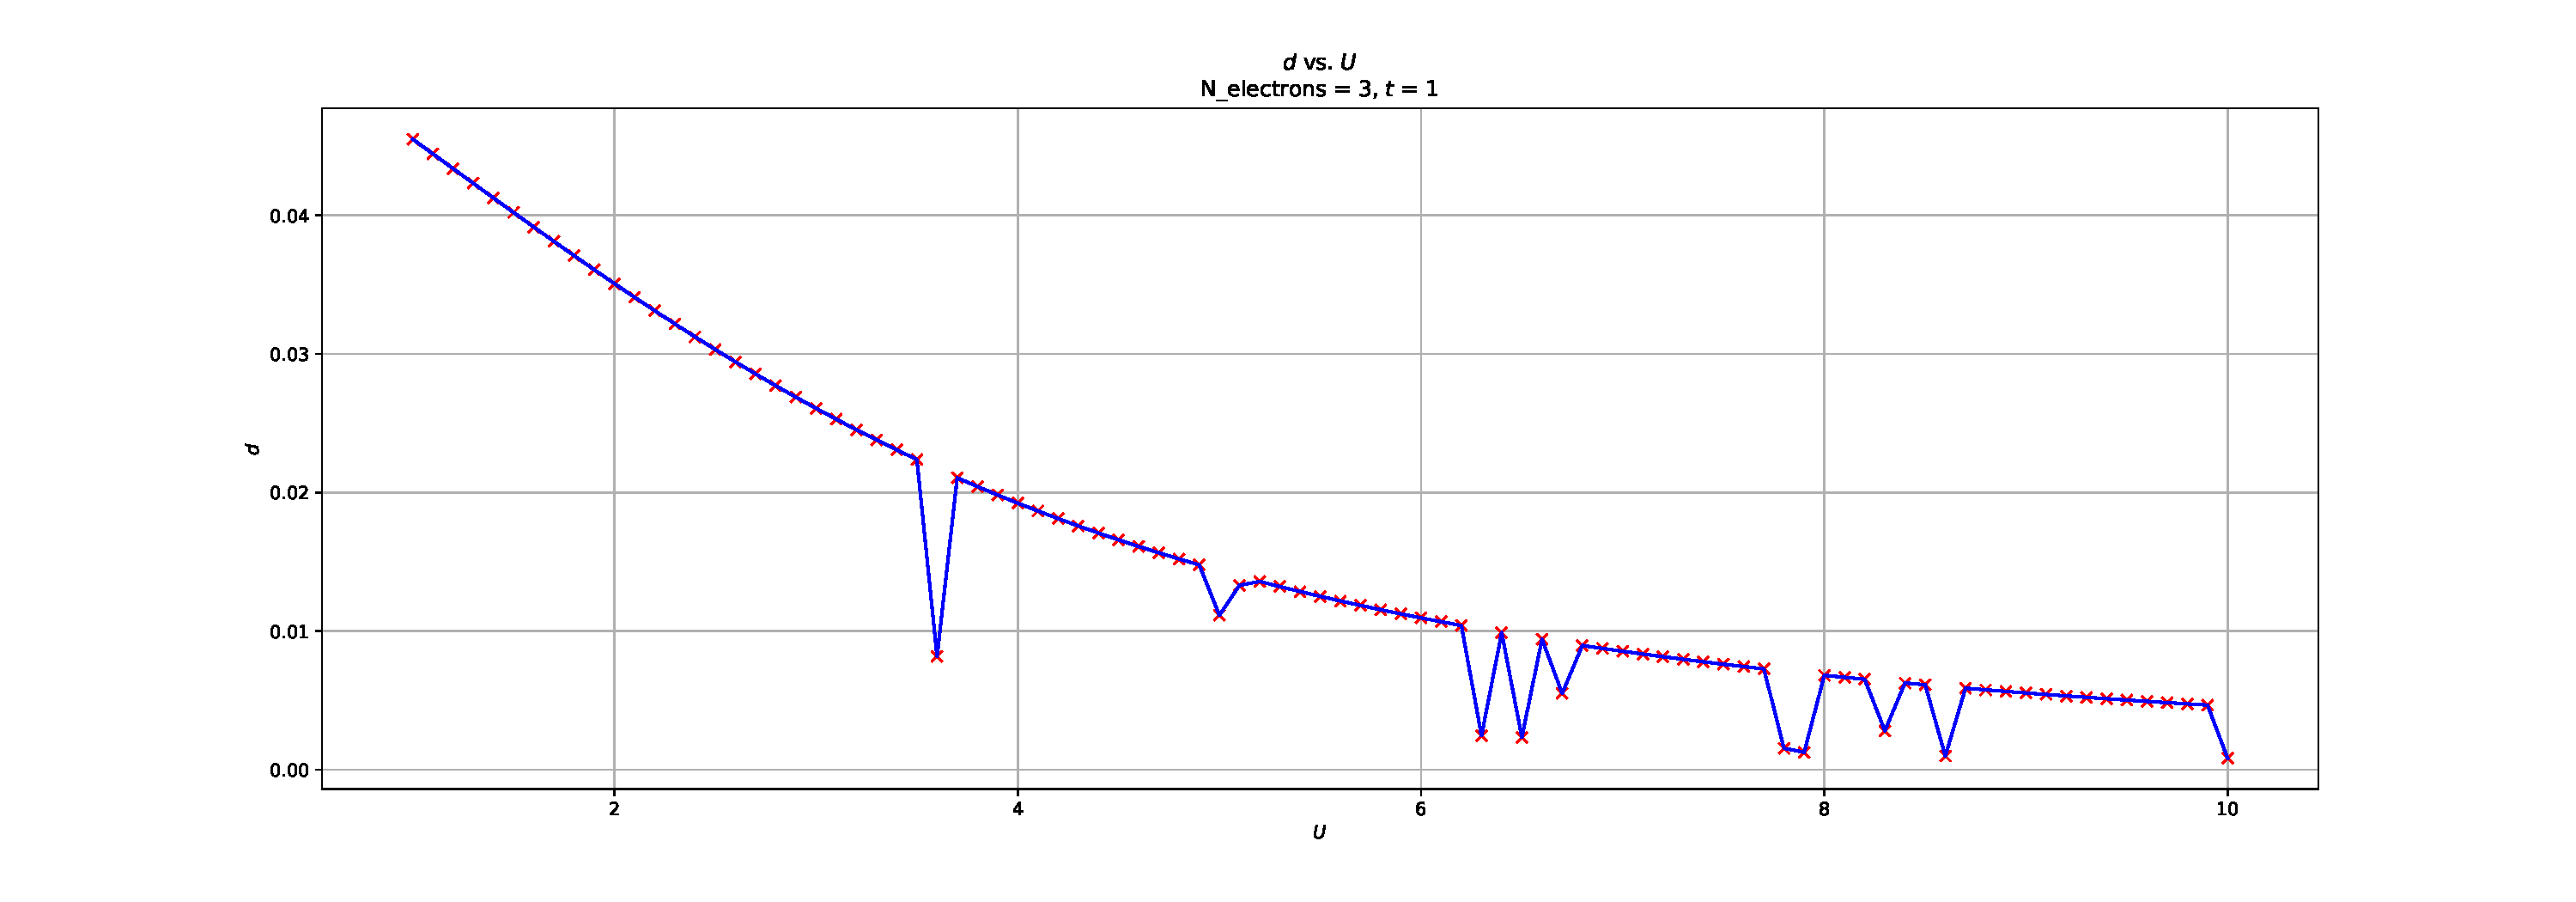
\includegraphics[trim = 5cm 0cm 5cm 0cm, clip, width=1.0\linewidth]{N3_t1/plot_dUi_N3_t1.0.pdf}
		\end{minipage}
		\begin{minipage}[t]{0.44\textwidth}
			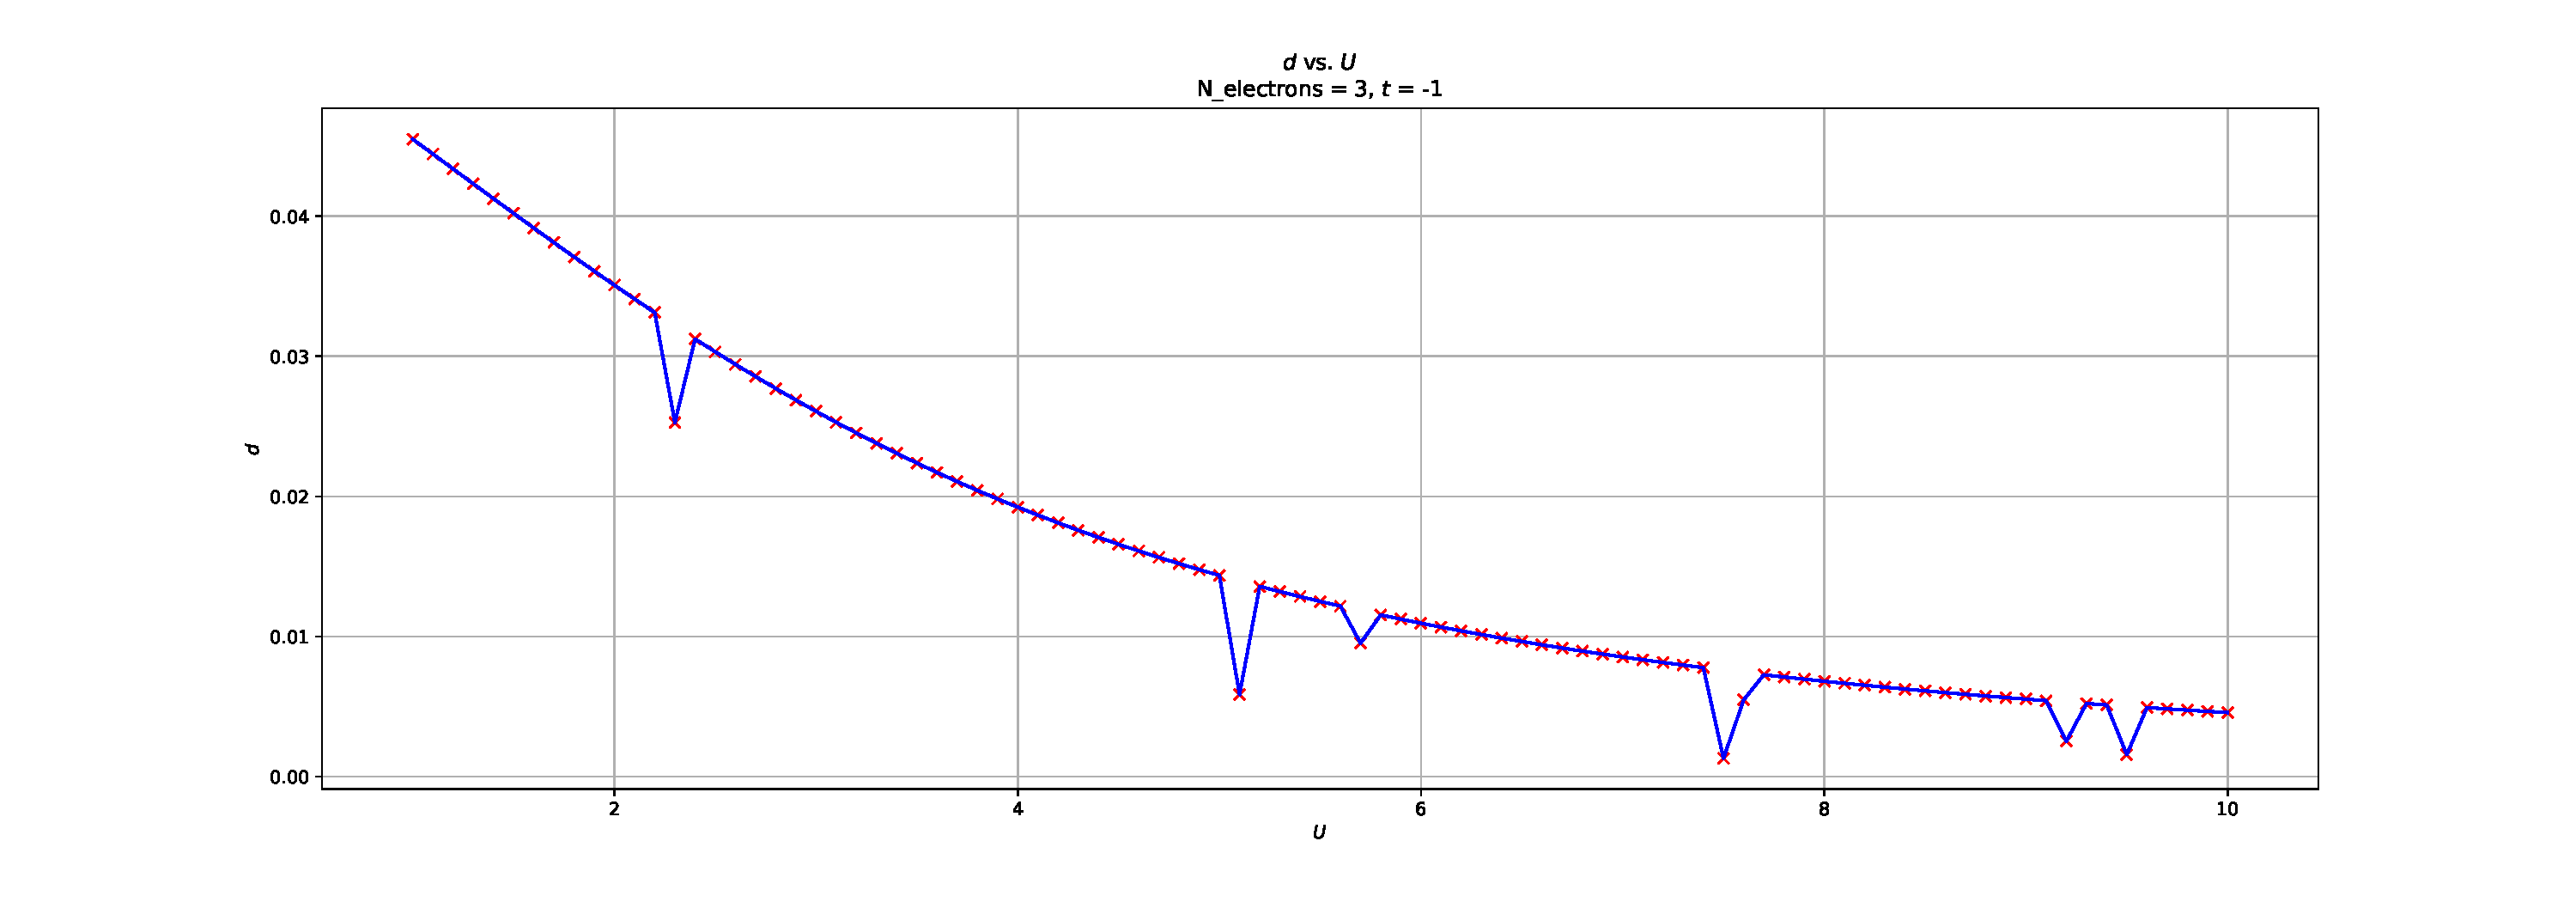
\includegraphics[trim = 5cm 0cm 5cm 0cm, clip, width=1.0\linewidth]{N3_t-1/plot_dUi_N3_t-1.0.pdf}
		\end{minipage}
		
		\begin{minipage}[t]{0.44\textwidth}
			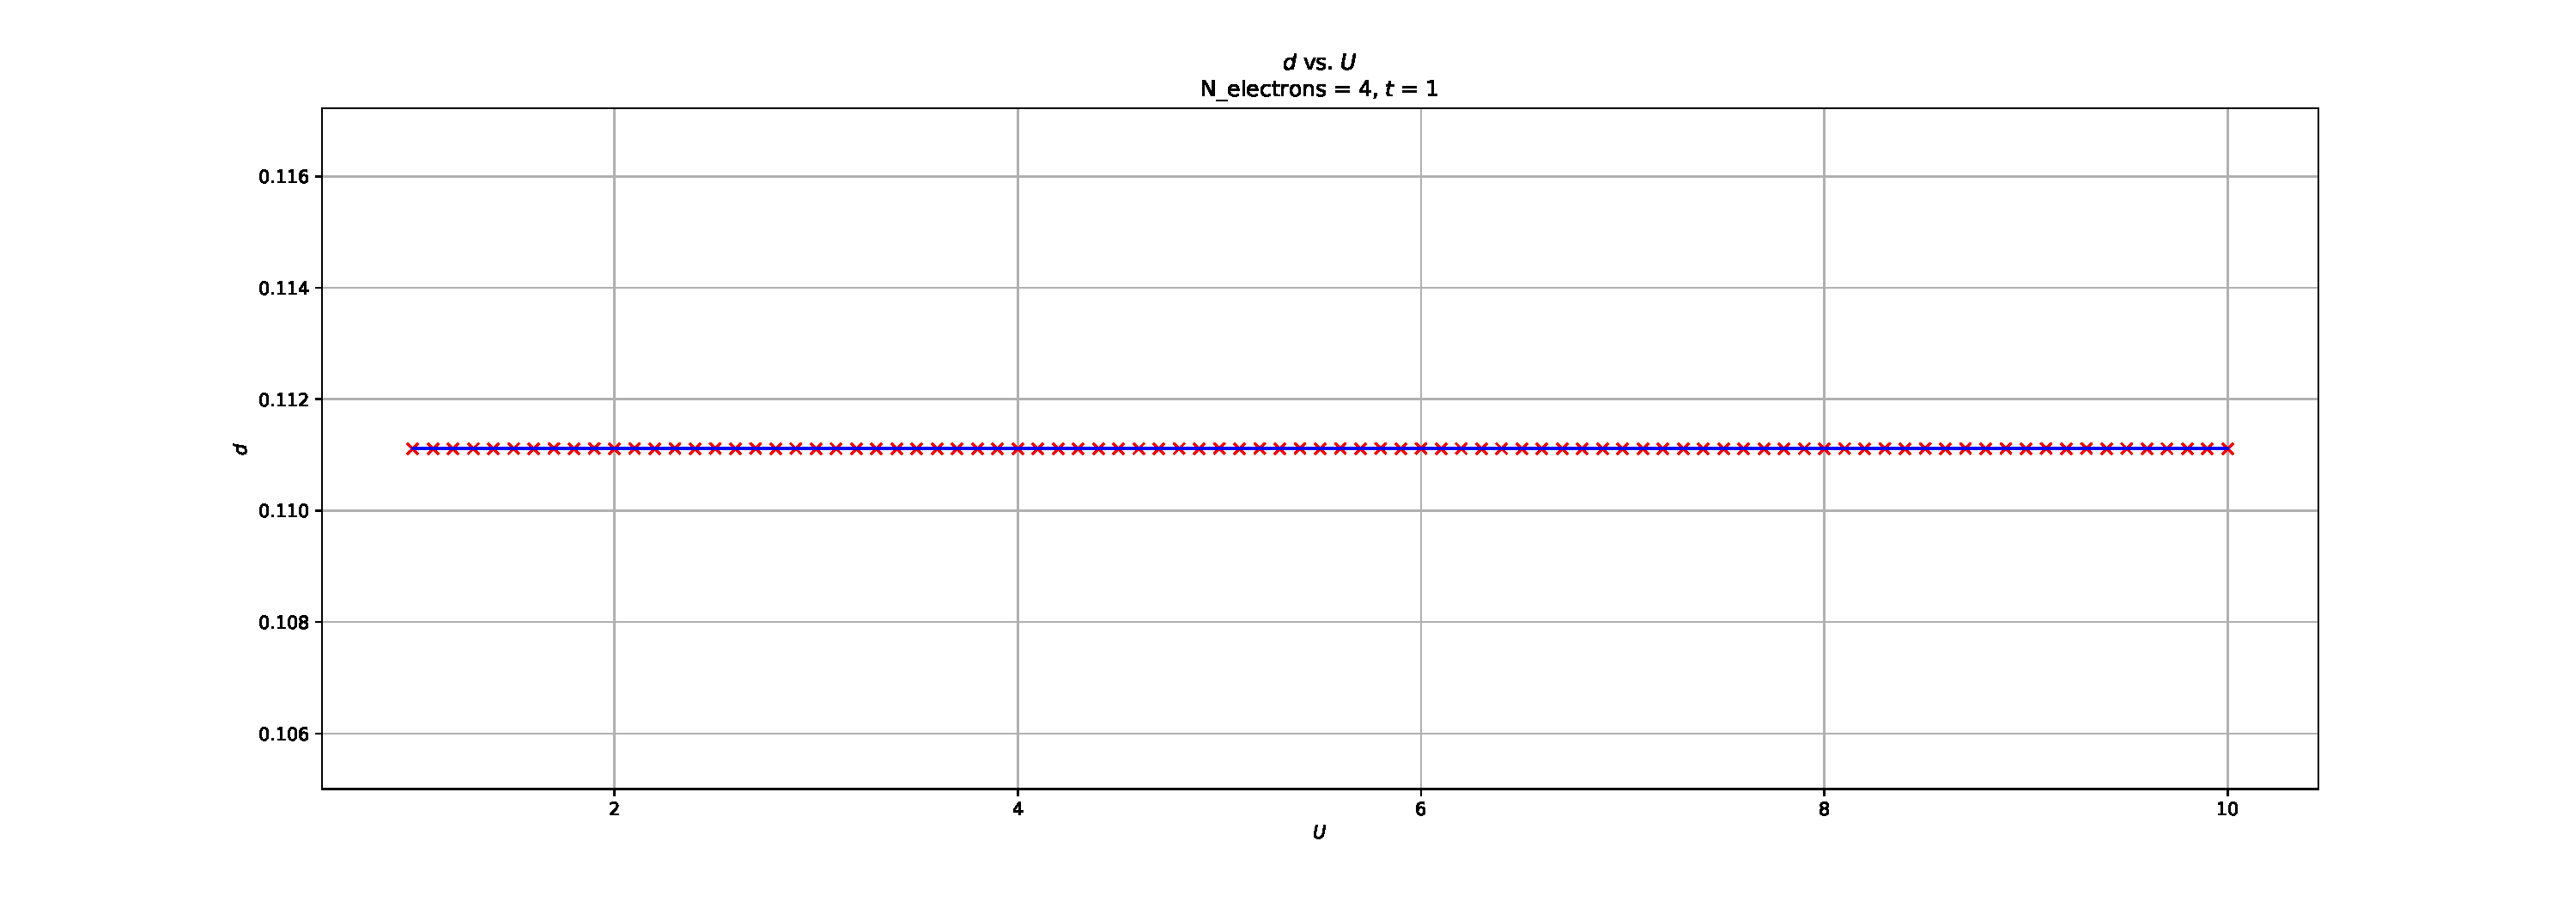
\includegraphics[trim = 5cm 0cm 5cm 0cm, clip, width=1.0\linewidth]{N4_t1/plot_dUi_N4_t1.0.pdf}
		\end{minipage}
		\begin{minipage}[t]{0.44\textwidth}
			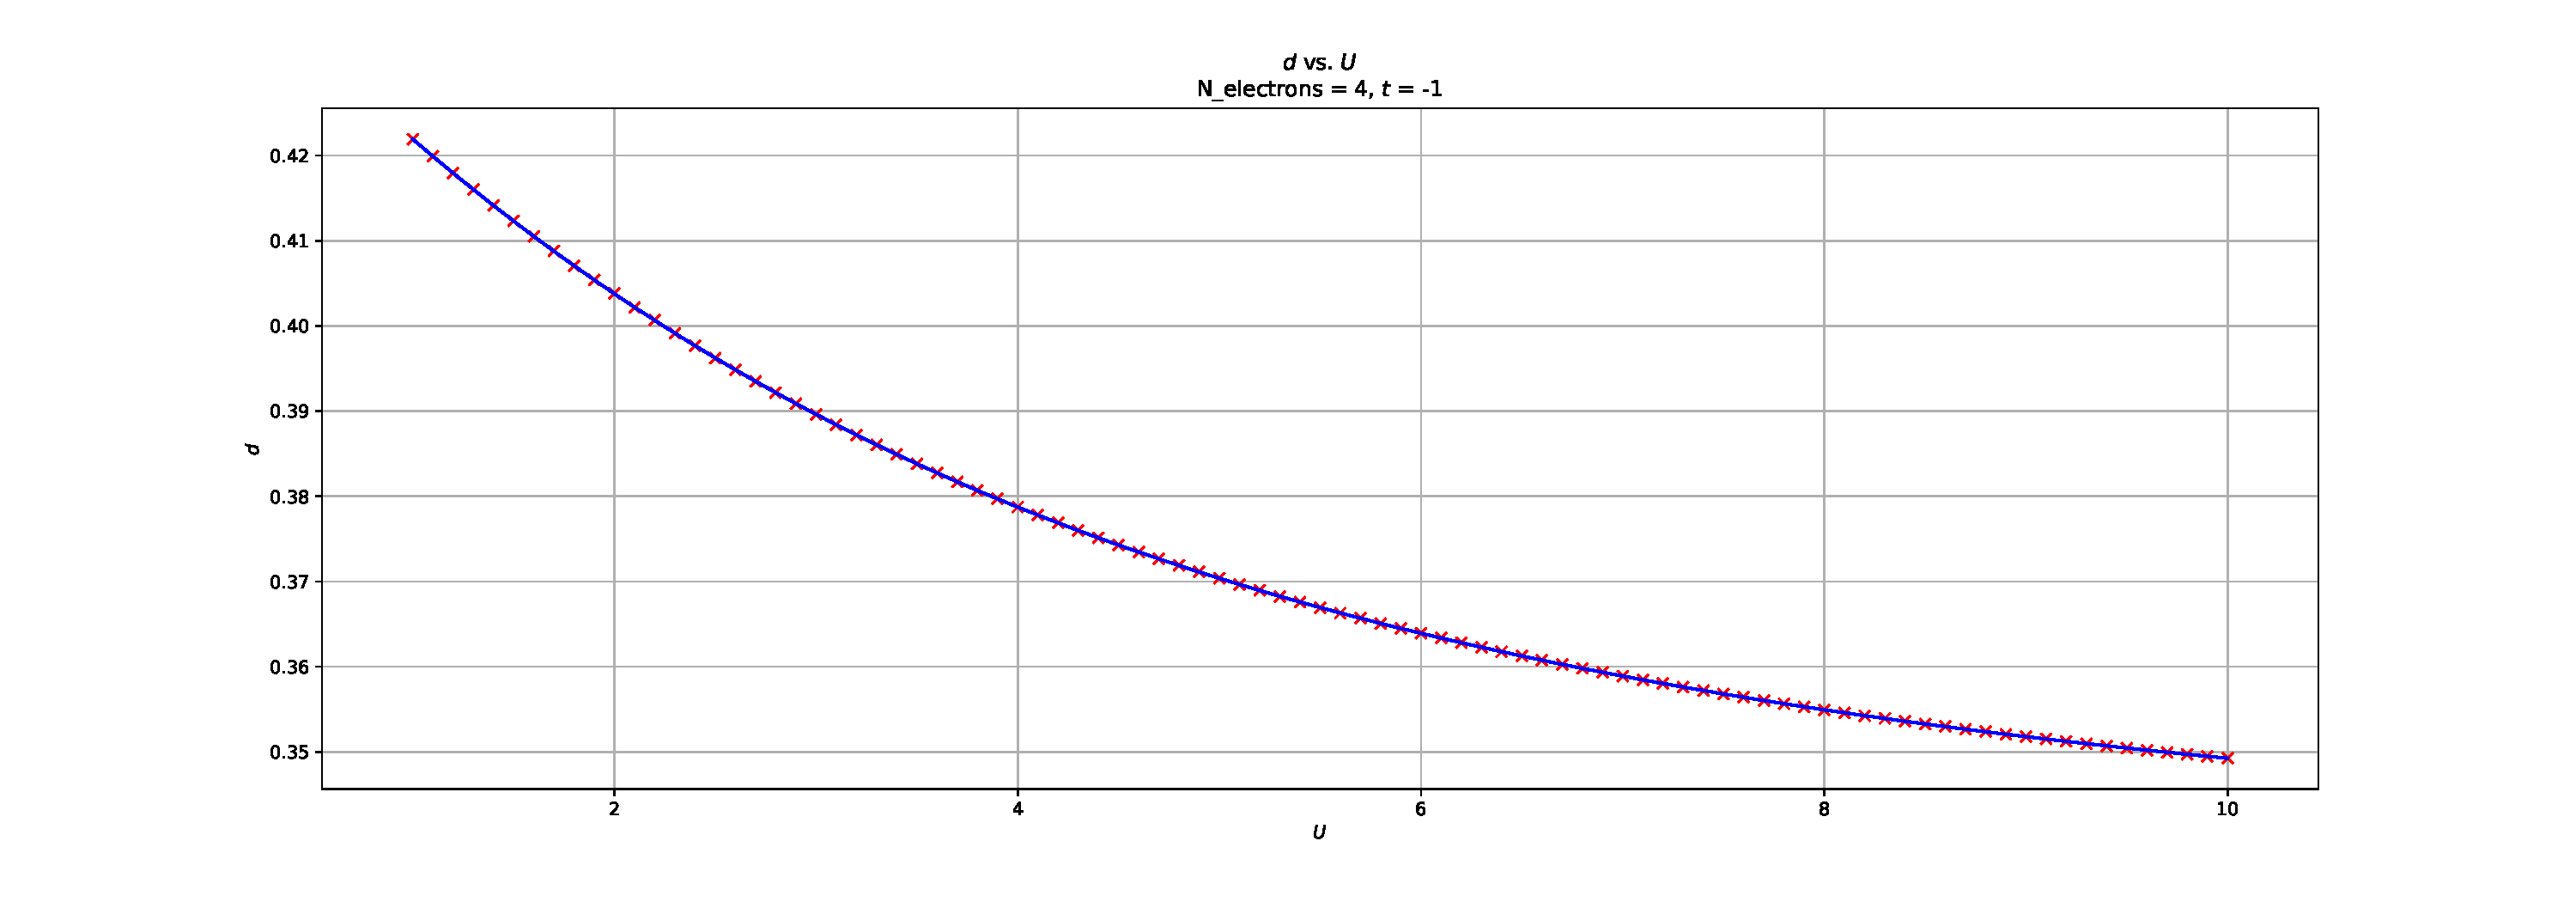
\includegraphics[trim = 5cm 0cm 5cm 0cm, clip, width=1.0\linewidth]{N4_t-1/plot_dUi_N4_t-1.0.pdf}
		\end{minipage}
	\end{center}	
\end{frame}

\begin{frame}\frametitle{E$_i$ vs. U}
	\begin{center}
		\begin{minipage}[t]{0.44\textwidth}
			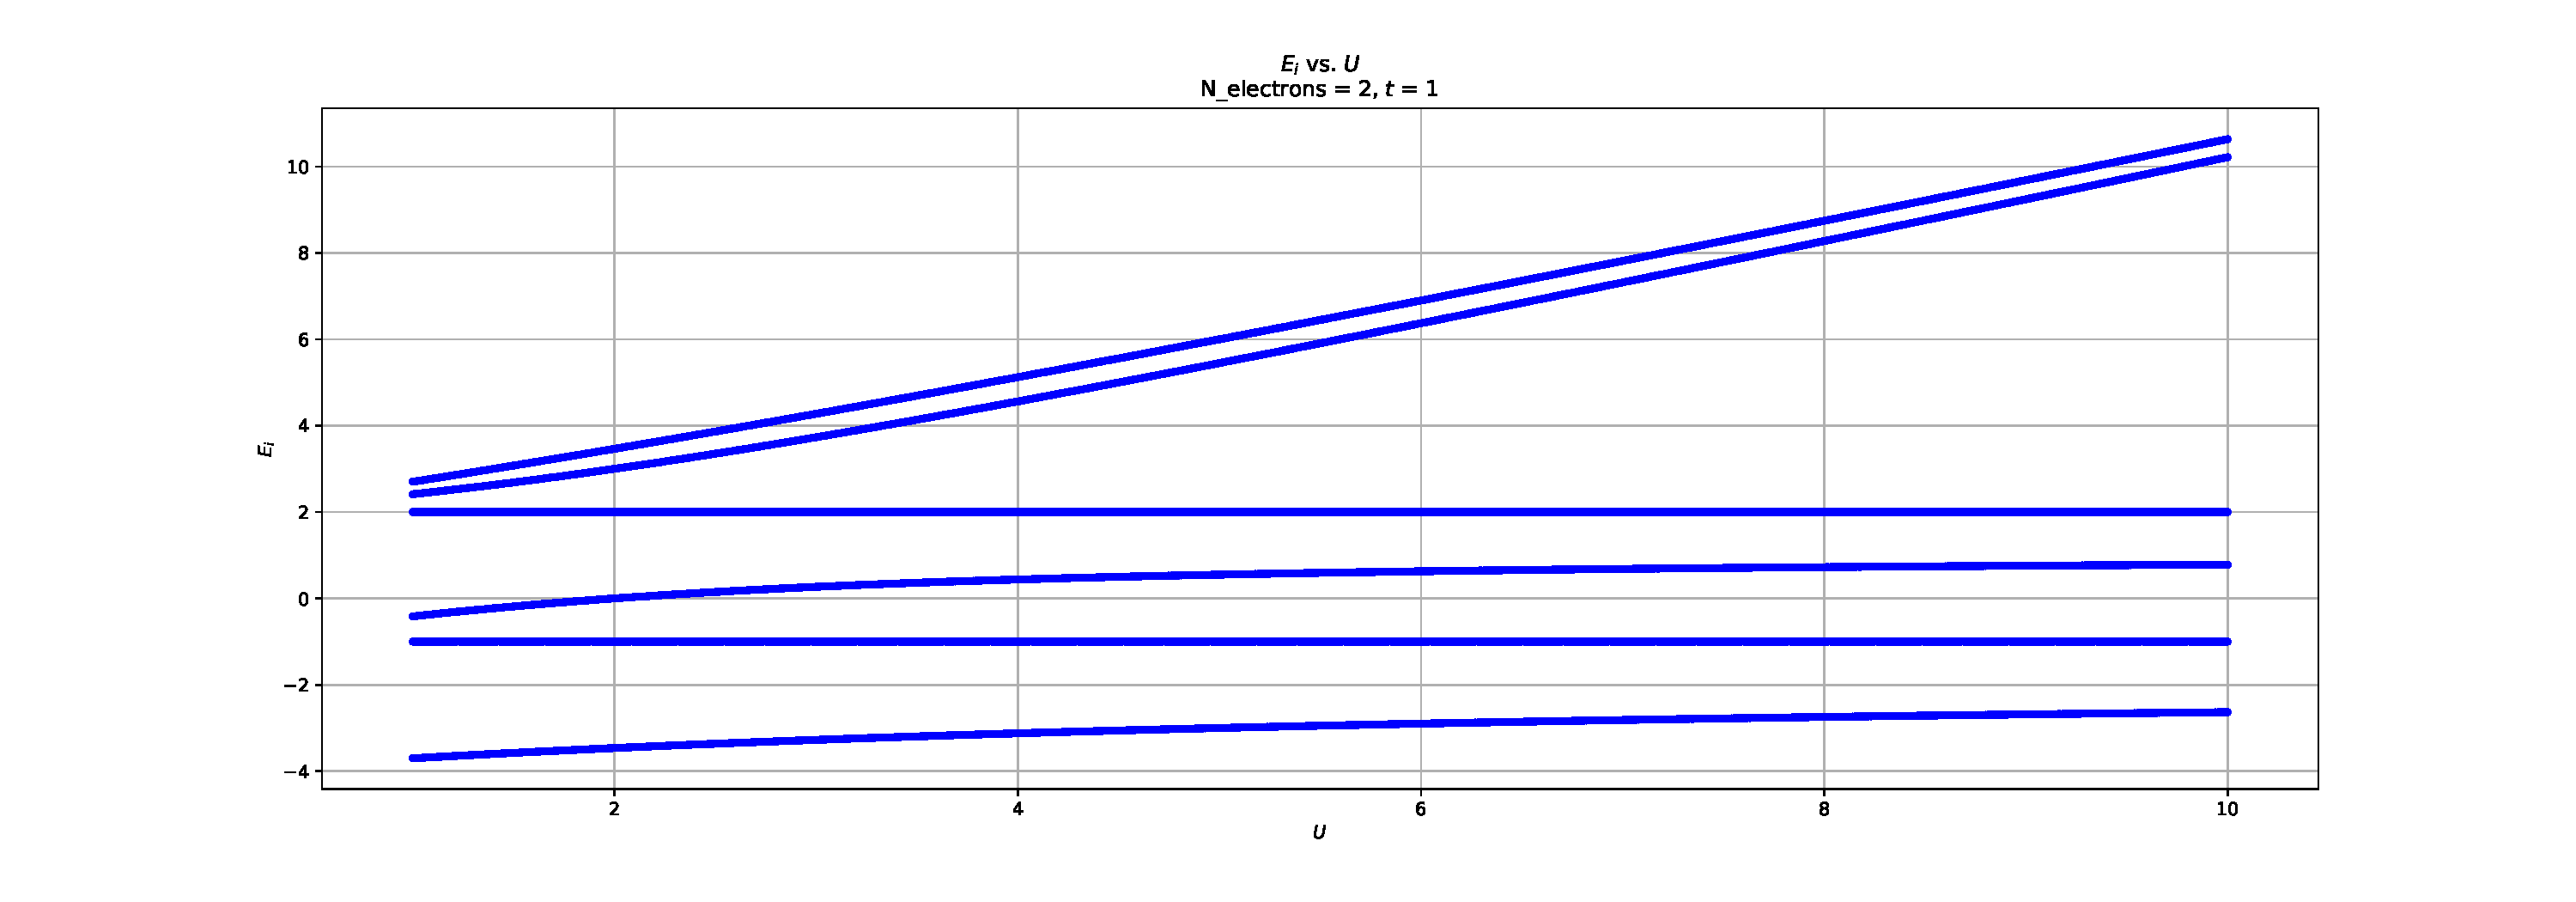
\includegraphics[trim = 5cm 0cm 5cm 0cm, clip, width=1.0\linewidth]{N2_t1/plot_EiUi_N2_t1.0.pdf}
		\end{minipage}
		\begin{minipage}[t]{0.44\textwidth}
			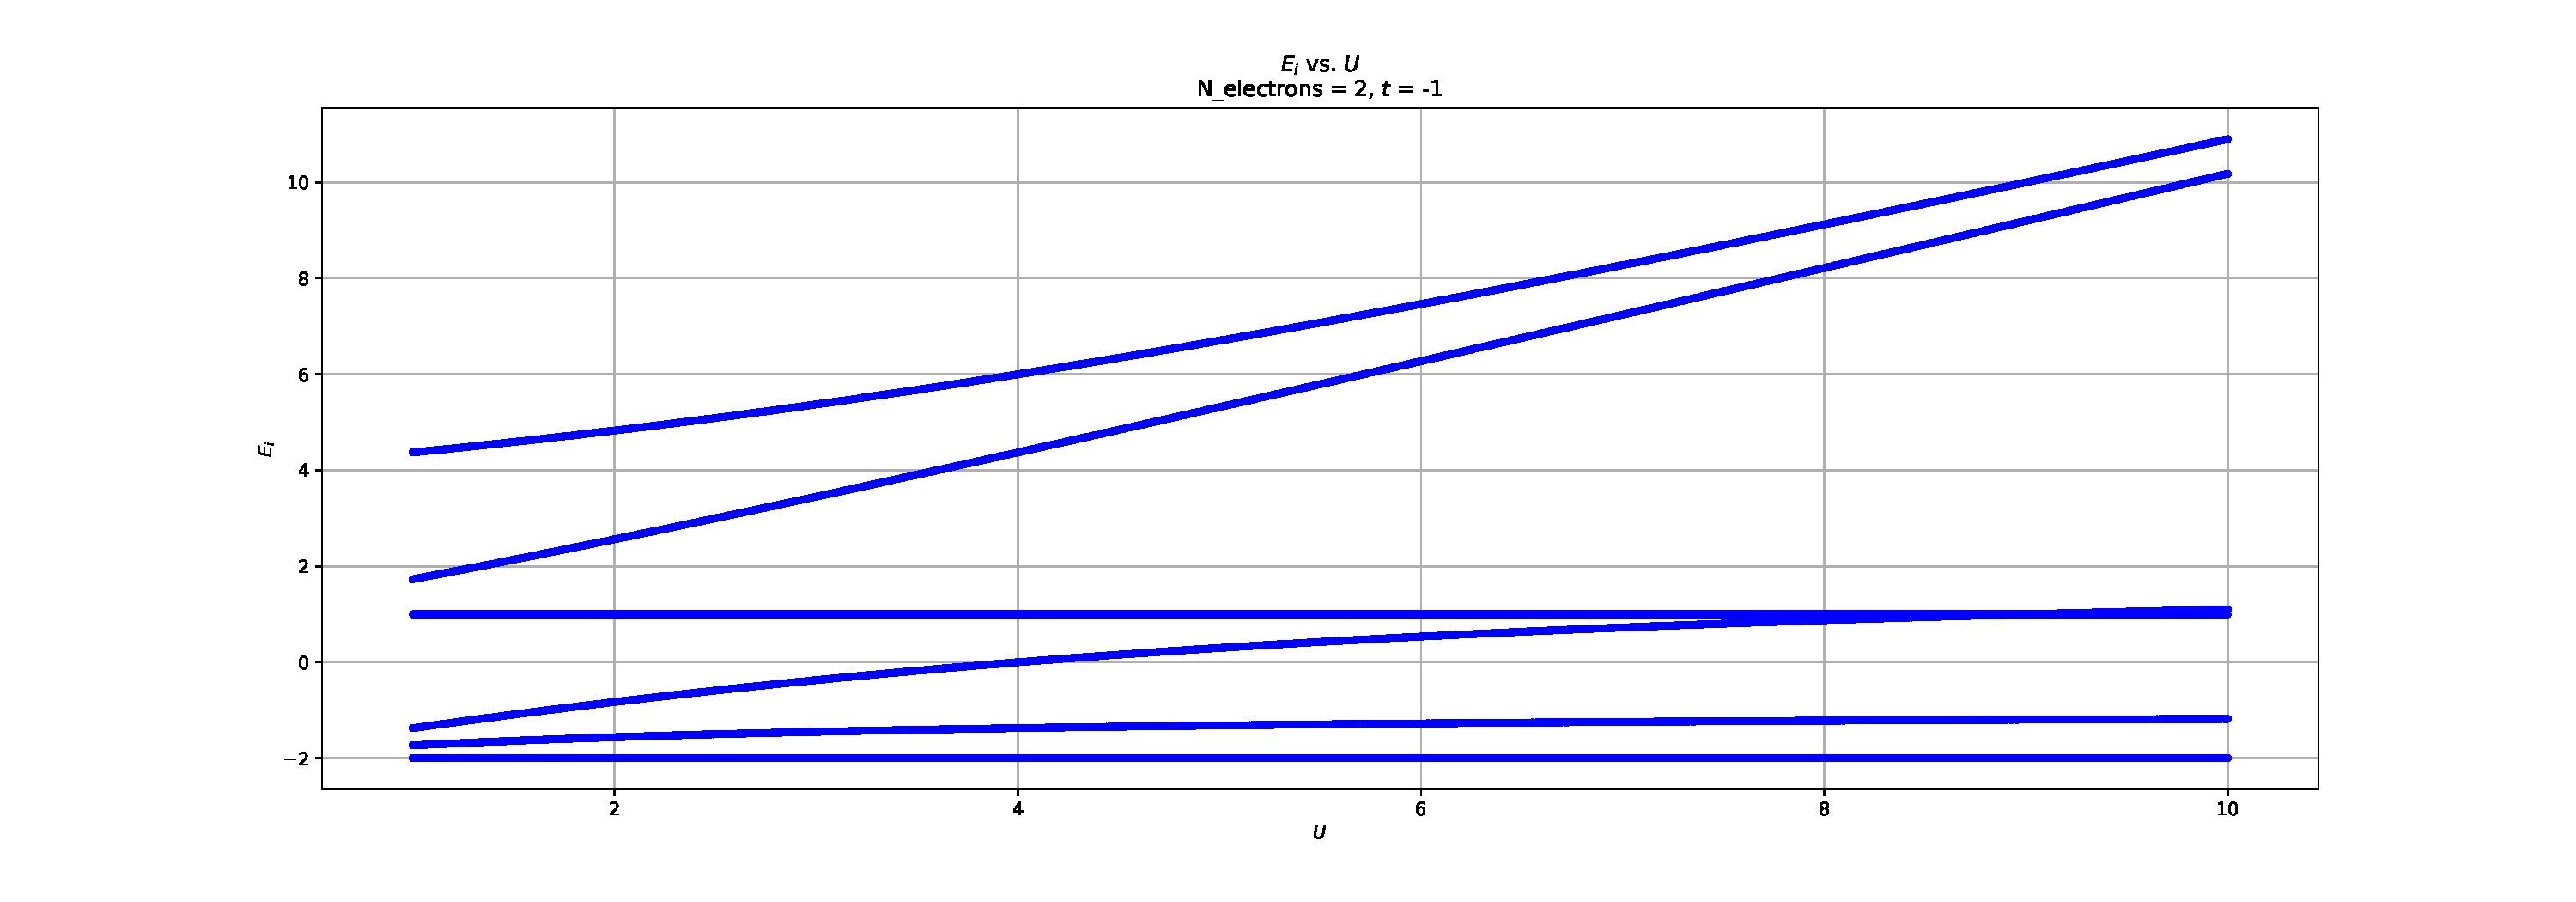
\includegraphics[trim = 5cm 0cm 5cm 0cm, clip, width=1.0\linewidth]{N2_t-1/plot_EiUi_N2_t-1.0.pdf}
		\end{minipage}
		
		\begin{minipage}[t]{0.44\textwidth}
			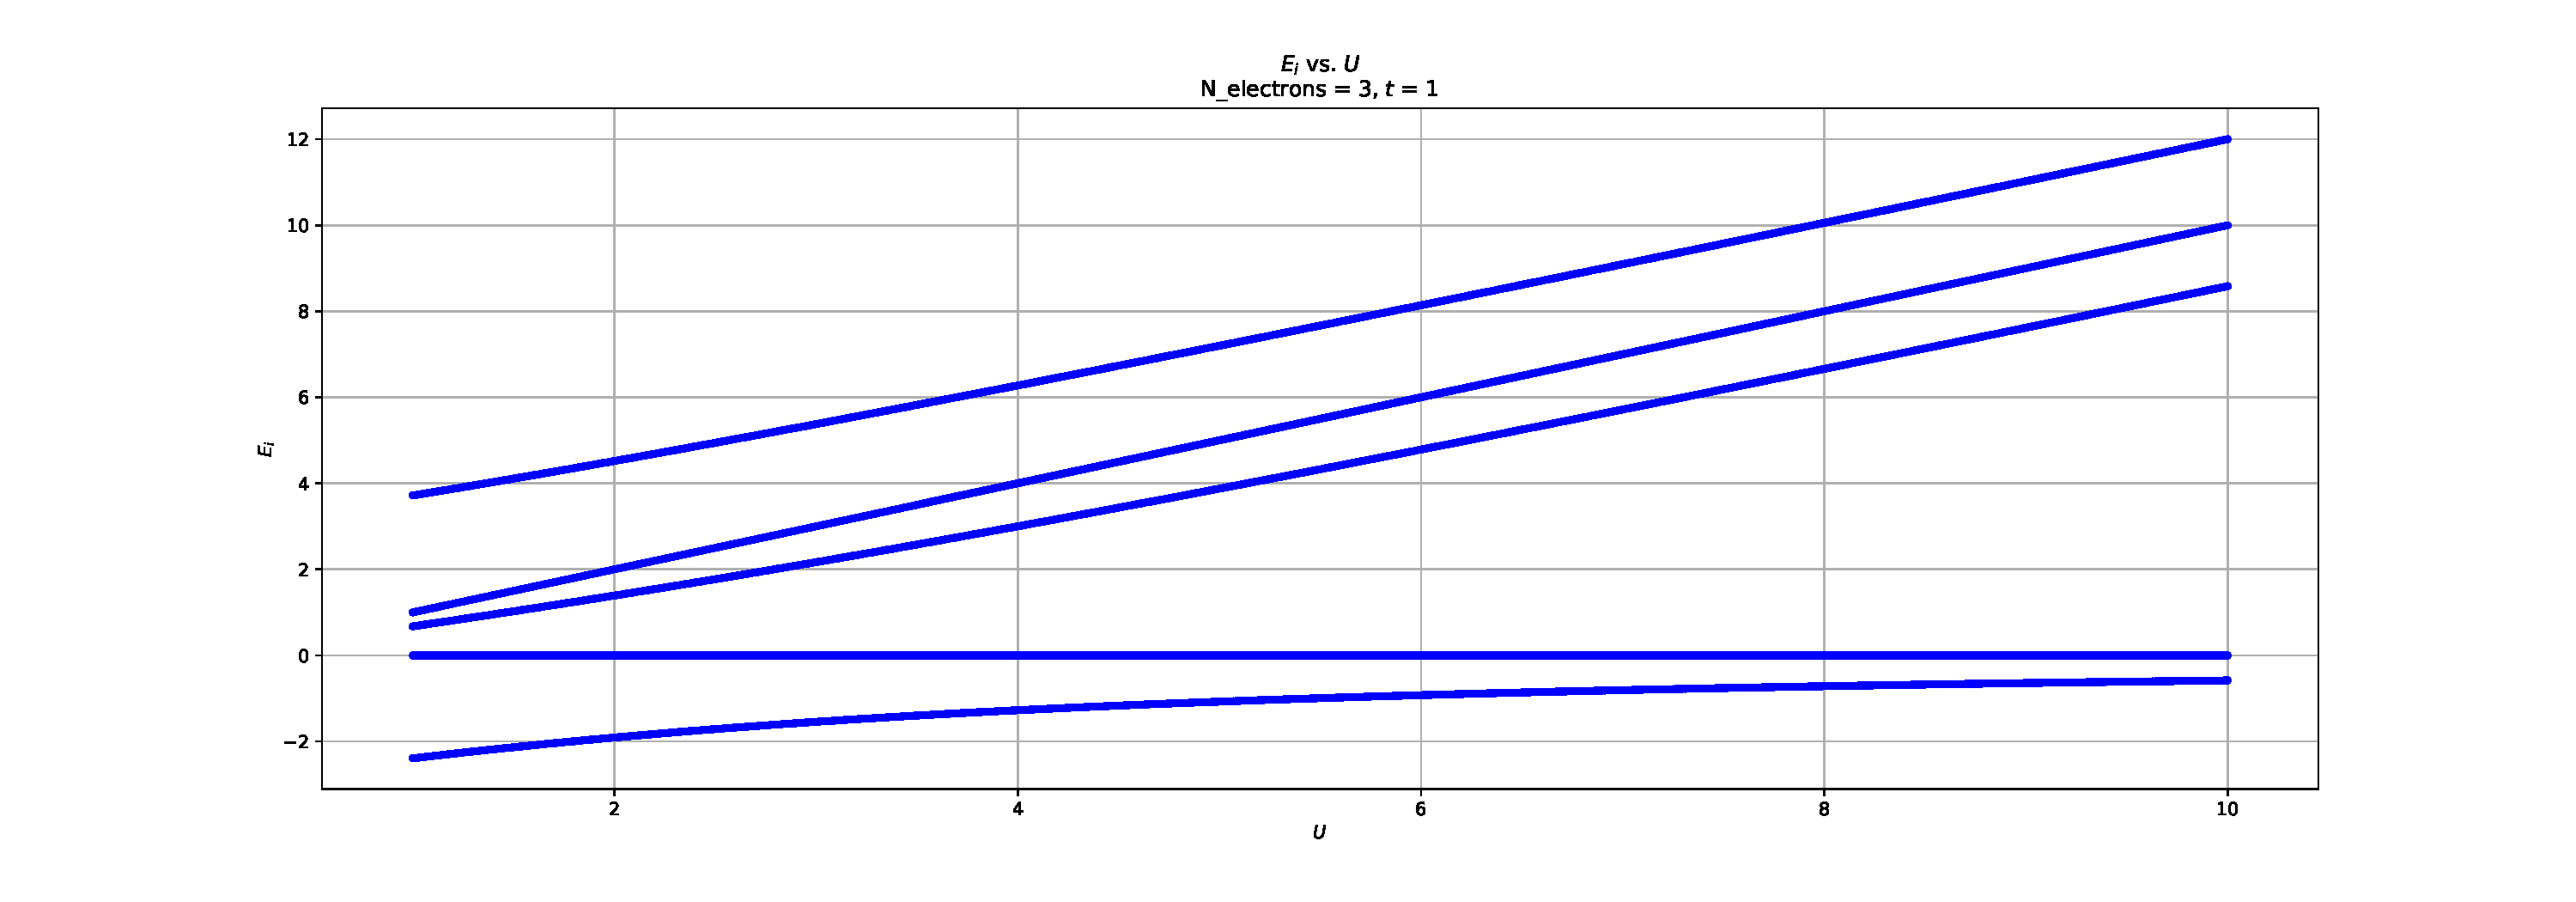
\includegraphics[trim = 5cm 0cm 5cm 0cm, clip, width=1.0\linewidth]{N3_t1/plot_EiUi_N3_t1.0.pdf}
		\end{minipage}
		\begin{minipage}[t]{0.44\textwidth}
			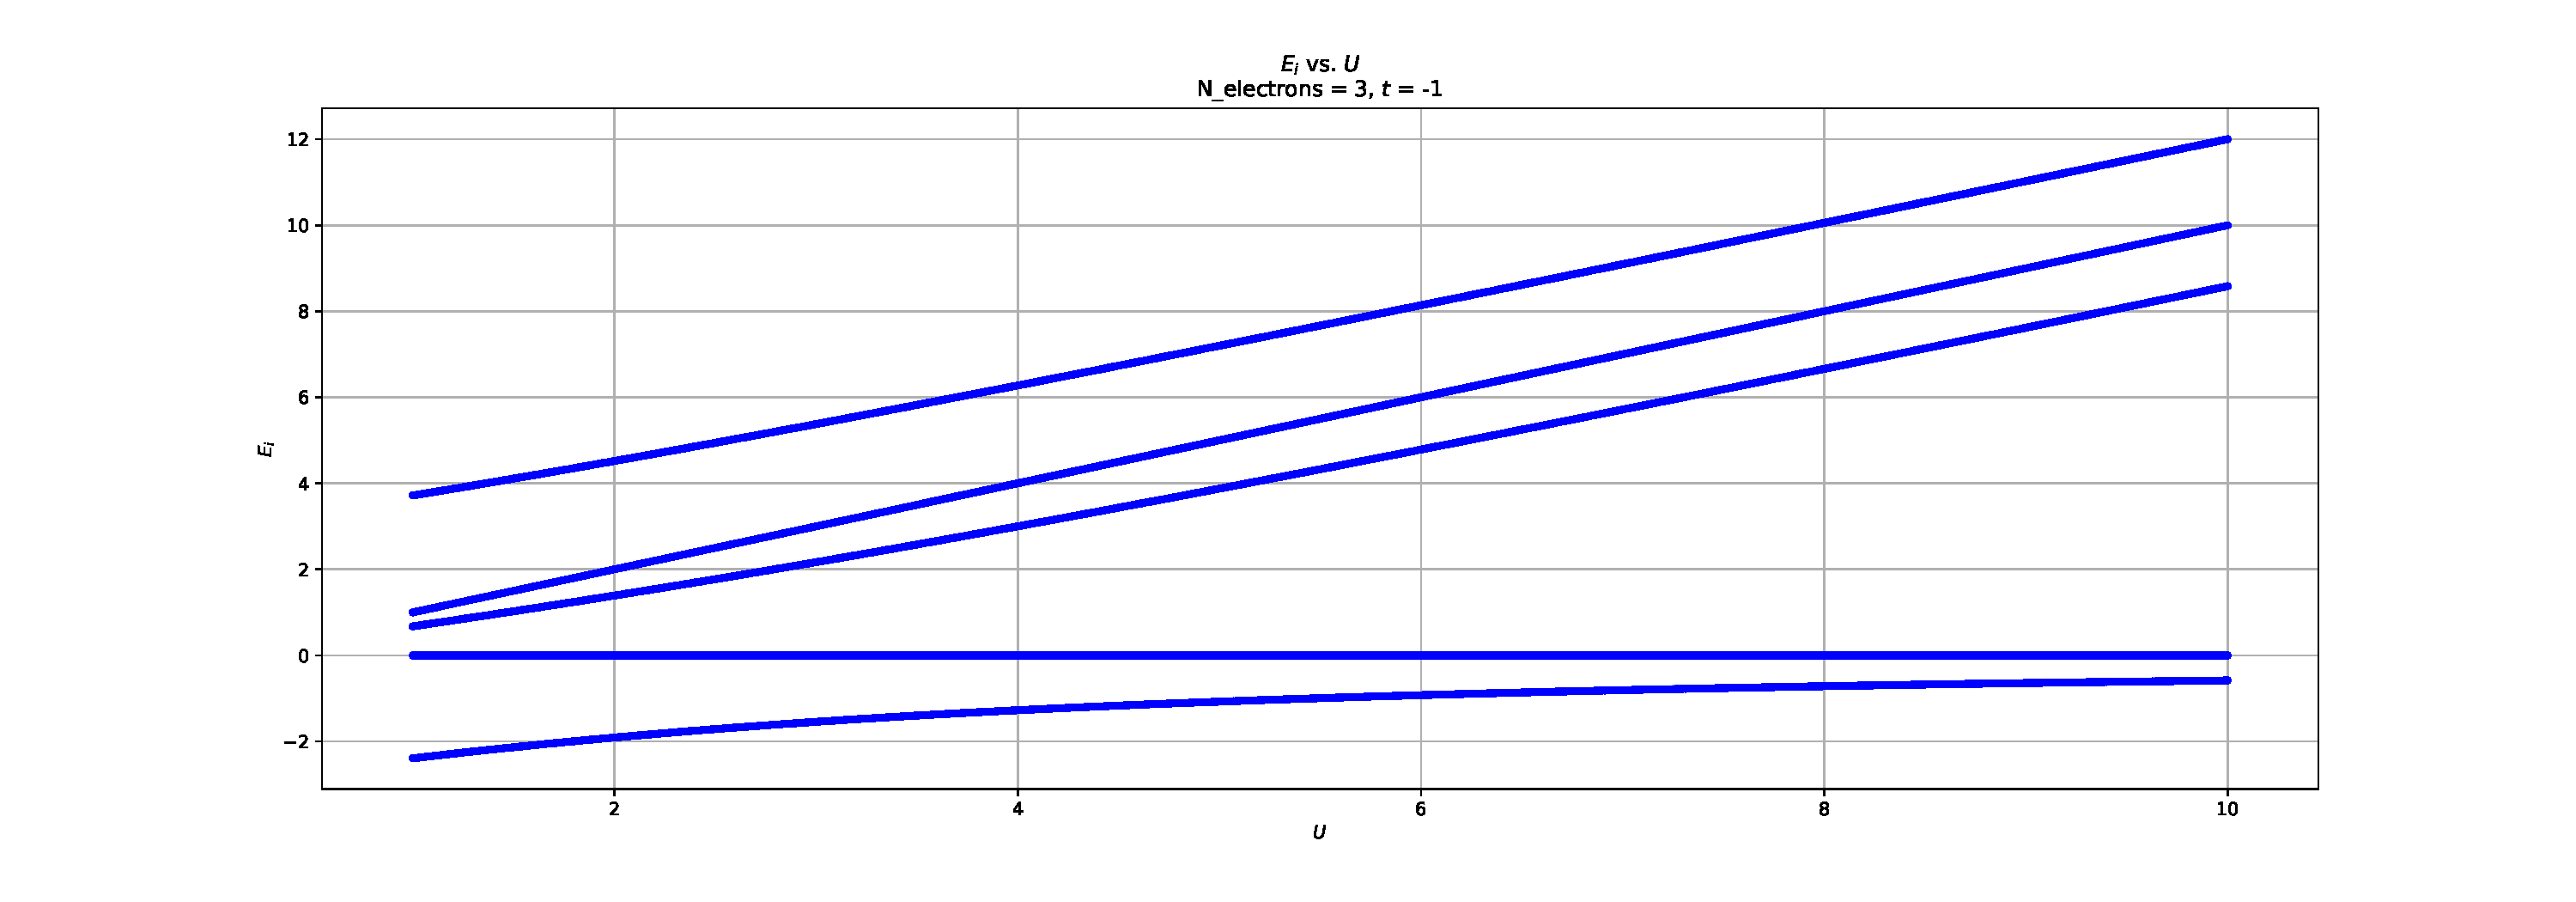
\includegraphics[trim = 5cm 0cm 5cm 0cm, clip, width=1.0\linewidth]{N3_t-1/plot_EiUi_N3_t-1.0.pdf}
		\end{minipage}
		
		\begin{minipage}[t]{0.44\textwidth}
			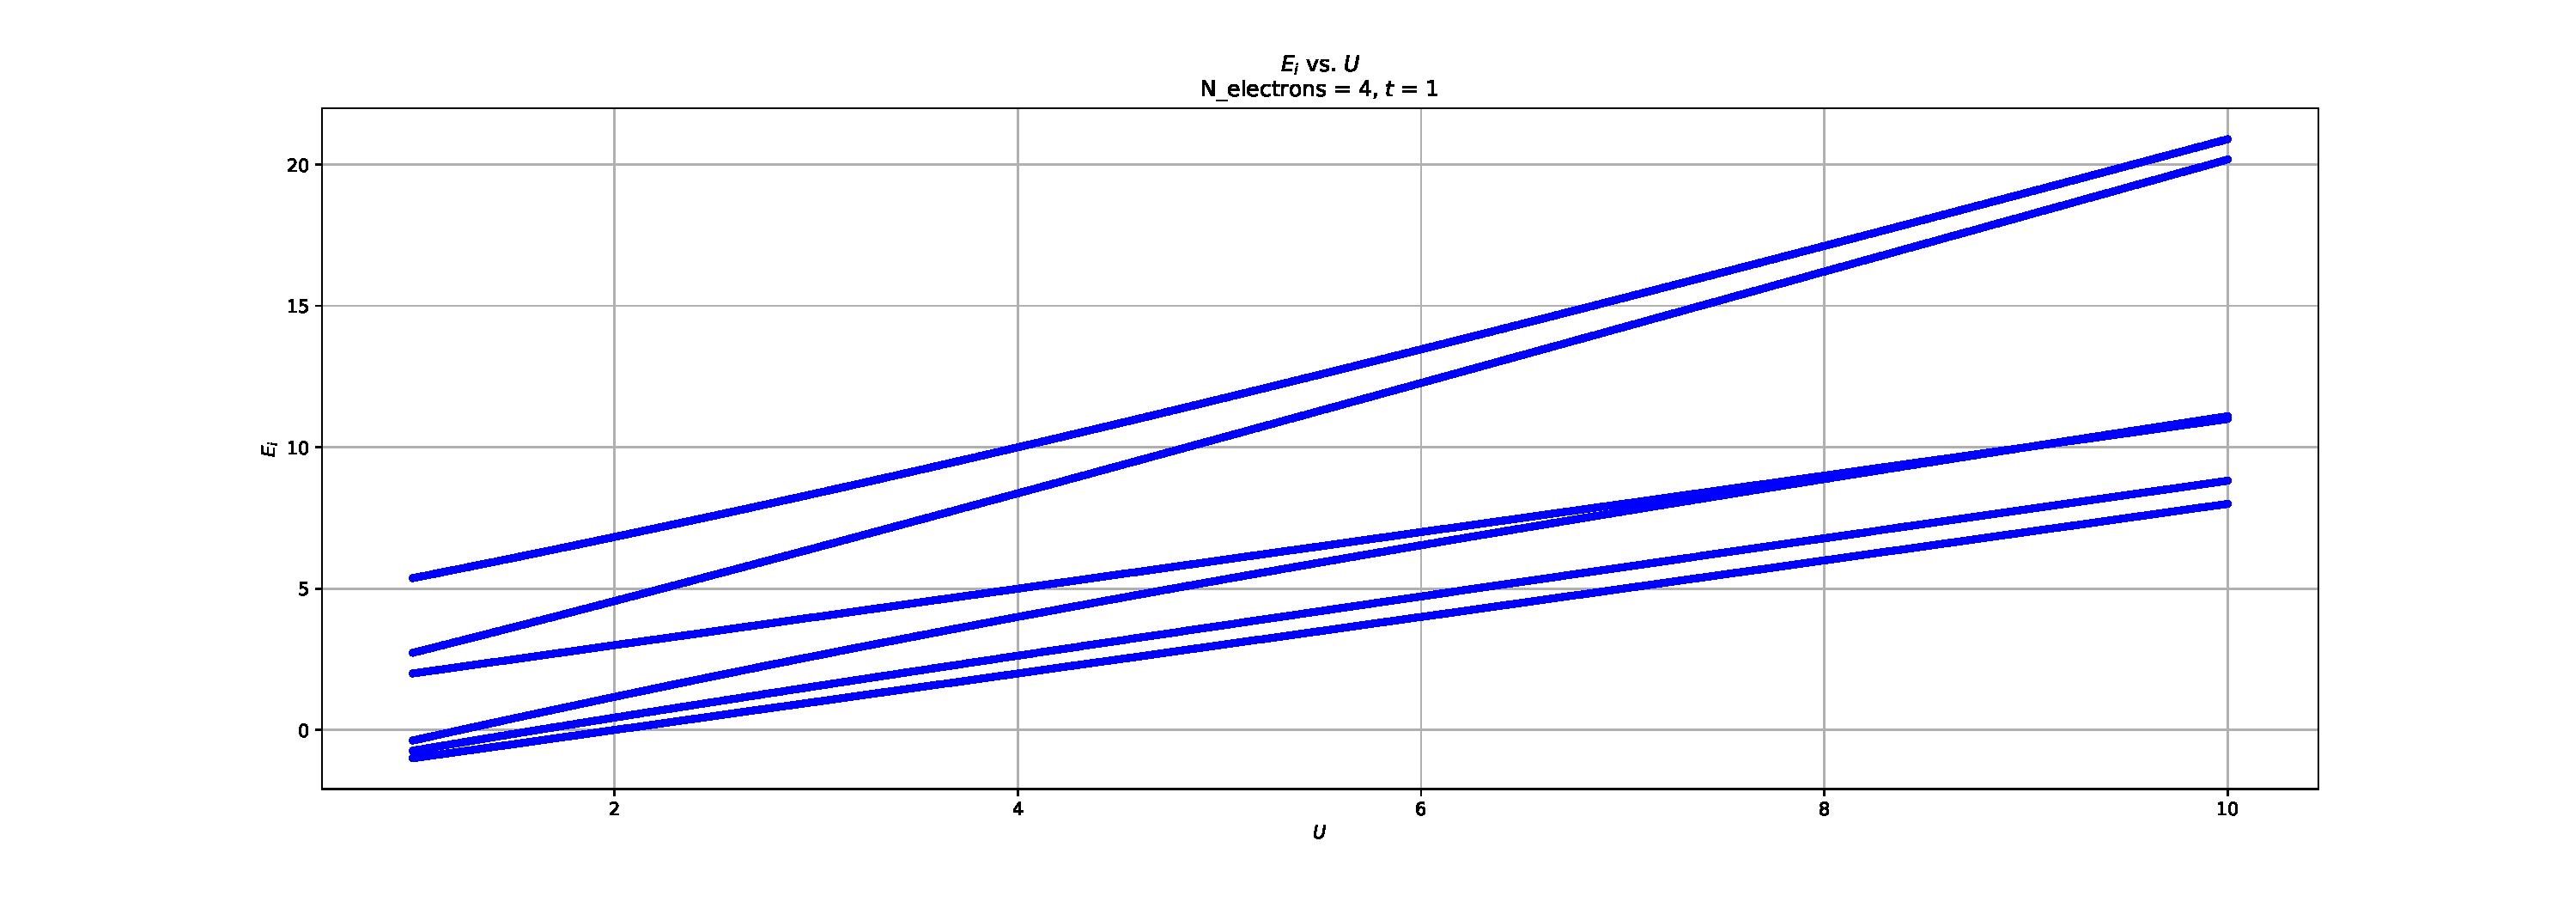
\includegraphics[trim = 5cm 0cm 5cm 0cm, clip, width=1.0\linewidth]{N4_t1/plot_EiUi_N4_t1.0.pdf}
		\end{minipage}
		\begin{minipage}[t]{0.44\textwidth}
			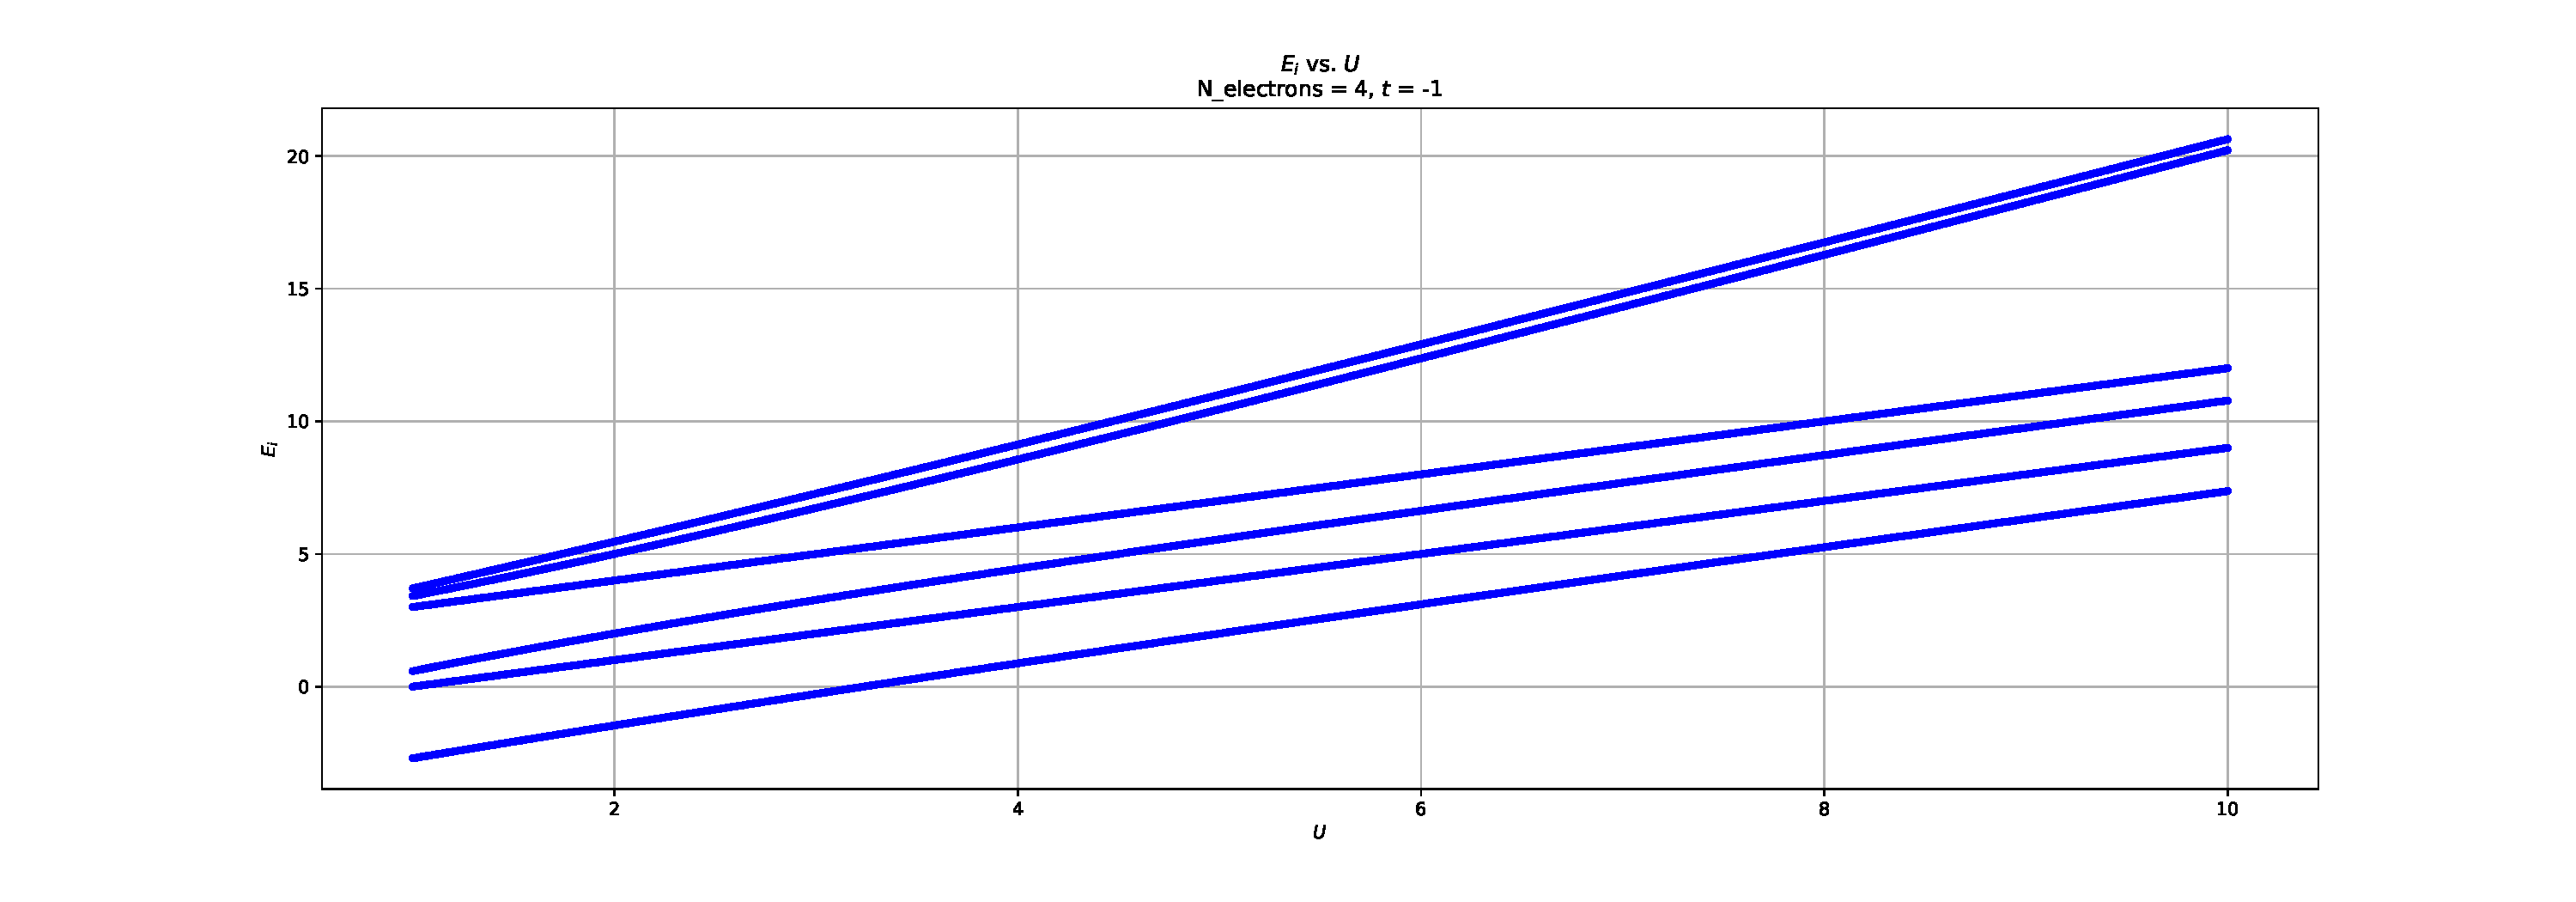
\includegraphics[trim = 5cm 0cm 5cm 0cm, clip, width=1.0\linewidth]{N4_t-1/plot_EiUi_N4_t-1.0.pdf}
		\end{minipage}
	\end{center}	
\end{frame}

\setbeamertemplate{headline}{%
}
\end{document}